\begin{center}
	\fbox{\textbf{Resolução da Lista 02}}
\end{center}
\begin{tcolorbox}[
	enhanced,
	sharp corners,
	boxrule=0.5pt,
	colback=white, 
	colframe=black,         
	width=1\textwidth,
	%fontupper=\itshape
	]%
	\textbf{Resumo:} Este documento apresenta a resolução detalhada da segunda lista de exercícios da disciplina de Variedades Diferenciáveis. O conteúdo foca na aplicação de conceitos de espaços tangentes, fibrados tangentes e a análise de campos vetoriais em variedades suaves. São explorados a representação coordenada de aplicações em esferas, a estrutura de variedades de espaços projetivos, a construção de atlas para o fibrado tangente $TM$ e o cálculo de colchetes de Lie para campos vetoriais em $\mathbb{R}^3$.
\end{tcolorbox}
%%%% QUESTÃO 01 %%%%
\questao{
	Considere a aplicação antípoda $A : \mathbb{S}^n \to \mathbb{S}^n$ definida por $A(p) = -p$, para cada $p \in \mathbb{S}^n$.
	\begin{enumerate}[label=(\alph*)]
		\item Calcule a representação coordenada $\hat{A}$ de $A$ em coordenadas estereográficas.
		\item Use a representação coordenada $\hat{A}$ de $A$ obtida para mostrar que $A$ é suave.
	\end{enumerate}
}
\solucao{
	
	\textbf{Análise do Enunciado}
	\begin{itemize}
		\item \textbf{Hipóteses:} $A$ é a aplicação antípoda em $\mathbb{S}^n$.
		\item \textbf{Tese (a):} Expressar $\hat{A} = \phi_S \circ A \circ \phi_N^{-1}$ analiticamente.
		\item \textbf{Tese (b):} Confirmar a suavidade de $A$ via representação coordenada.
	\end{itemize}
	
	\textbf{Fundamentação Teórica}
	
	Utilizamos o atlas de projeções estereográficas construído na \textbf{Questão 3 da Lista 01}. Especificamente, as cartas $\phi_N$ (polo norte) e $\phi_S$ (polo sul) e a expressão de $\phi_N^{-1} : \mathbb{R}^n \to \mathbb{S}^n$:
	\begin{equation*}
		\phi_N^{-1}(u) = \frac{\left(2u^1, \dots, 2u^n, |u|^2-1\right)}{|u|^2+1}.
	\end{equation*}
	Embora a suavidade de $A$ tenha sido estabelecida globalmente na \textbf{Questão 20 da Lista 01} (via restrição de aplicação linear no espaço ambiente), a tese aqui exige a verificação local através da representação coordenada $\hat{A}$.
	
	\textbf{Desenvolvimento Formal}
	
	\textbf{(a)} Para $u \in \mathbb{R}^n$, a representação coordenada $\hat{A} = \phi_S \circ A \circ \phi_N^{-1}$ é obtida pela seguinte composição:
	\begin{enumerate}
		\item $\phi_N^{-1}(u) = p = \left( \frac{2u^1}{|u|^2+1}, \dots, \frac{2u^n}{|u|^2+1}, \frac{|u|^2-1}{|u|^2+1} \right)$.
		\item $A(p) = -p = (y^1, \dots, y^{n+1}) = \left( \frac{-2u^1}{|u|^2+1}, \dots, \frac{-2u^n}{|u|^2+1}, \frac{1-|u|^2}{|u|^2+1} \right)$.
	\end{enumerate}
	Aplicando $\phi_S$ ao ponto $A(p)$, temos que $\hat{A}^i(u) = \frac{y^i}{1+y^{n+1}}$ para $i=1,\dots,n$. Calculando o denominador:
	\begin{align*}
		1+y^{n+1} &= 1 + \frac{1-|u|^2}{|u|^2+1} = \frac{|u|^2+1 + 1-|u|^2}{|u|^2+1} = \frac{2}{|u|^2+1}.
	\end{align*}
	Substituindo nas componentes:
	\begin{align*}
		\hat{A}^i(u) &= \frac{\dfrac{-2u^i}{|u|^2+1}}{\dfrac{2}{|u|^2+1}} = -u^i.
	\end{align*}
	Portanto, a representação coordenada é a aplicação linear:
	\begin{equation*}
		\boxed{\hat{A}(u) = -u}.
	\end{equation*}
	
	\textbf{(b)} Como $\hat{A} = -\text{Id}_{\mathbb{R}^n}$ é uma aplicação linear, ela é infinitamente diferenciável ($C^\infty$). Visto que as representações coordenadas de $A$ em qualquer par de cartas do atlas suave de $\mathbb{S}^n$ são composições de $\hat{A}$ com funções de transição suaves, a suavidade de $\hat{A}$ garante que $A$ é uma aplicação suave.
}
%%%% QUESTÃO 02 %%%%
\questao{
	Seja $F : \mathbb{R}^{n+1} \setminus \{0\} \to \mathbb{R}^{m+1} \setminus \{0\}$ uma função suave e homogênea de grau $d$ (isto é, existe $d \in \mathbb{Z}$ tal que $F(\lambda x) = \lambda^d F(x)$ para todo $\lambda \in \mathbb{R} \setminus \{0\}$ e qualquer $x \in \mathbb{R}^{n+1} \setminus \{0\}$). Prove que $f : \mathbb{RP}^n \to \mathbb{RP}^m$ definida por $f([x]) = [F(x)]$ está bem definida e é suave.
}
\solucao{
	
	\textbf{Análise do Enunciado}
	\begin{itemize}
		\item \textbf{Hipóteses:} $F$ é uma aplicação suave entre espaços euclidianos (menos a origem) e satisfaz a condição de homogeneidade $F(\lambda x) = \lambda^d F(x)$.
		\item \textbf{Tese 1:} a aplicação $f$ é bem definida, ou seja, a imagem de uma classe de equivalência $[x] \in \mathbb{RP}^n$ não depende do representante $x$ escolhido.
		\item \textbf{Tese 2:} $f$ é uma aplicação suave entre as variedades $\mathbb{RP}^n$ e $\mathbb{RP}^m$.
	\end{itemize}
	
	\textbf{Fundamentação Teórica}
	
	Recordamos a definição de $\mathbb{RP}^n$ como o espaço quociente $(\mathbb{R}^{n+1} \setminus \{0\}) / \sim$, onde $x \sim y \iff y = \lambda x$ para algum $\lambda \neq 0$. Conforme a \textbf{Questão 4 da Lista 01}, $\mathbb{RP}^n$ é uma variedade suave cujo atlas é composto pelas cartas $\phi_i : U_i \to \mathbb{R}^n$, onde $U_i = \{ [x] \in \mathbb{RP}^n : x^i \neq 0 \}$, dadas por:
	\begin{equation*}
		\phi_i([x]) = \left( \frac{x^1}{x^i}, \dots, \frac{x^{i-1}}{x^i}, \frac{x^{i+1}}{x^i}, \dots, \frac{x^{n+1}}{x^i} \right).
	\end{equation*}
	Uma aplicação $f : \mathbb{RP}^n \to \mathbb{RP}^m$ é suave se, para qualquer par de cartas $\phi_i$ em $\mathbb{RP}^n$ e $\psi_j$ em $\mathbb{RP}^m$, a representação coordenada $\hat{f} = \psi_j \circ f \circ \phi_i^{-1}$ for suave.
	
	\textbf{Desenvolvimento Formal}
	
	\textbf{1. Prova de que $f$ está bem definida:}
	Sejam $x, y \in \mathbb{R}^{n+1} \setminus \{0\}$ representantes da mesma classe de equivalência em $\mathbb{RP}^n$. Então, existe $\lambda \in \mathbb{R} \setminus \{0\}$ tal que $y = \lambda x$. Aplicando a função $F$:
	\begin{align*}
		f([y]) &= [F(y)] \\
		&= [F(\lambda x)] \\
		&= [\lambda^d F(x)] \quad (\text{por homogeneidade de } F).
	\end{align*}
	Como $F(x) \in \mathbb{R}^{m+1} \setminus \{0\}$ e $\lambda \neq 0$, segue que $\lambda^d \neq 0$. Assim, os vetores $F(x)$ e $\lambda^d F(x)$ são linearmente dependentes, o que implica que eles pertencem à mesma classe de equivalência no espaço projetivo $\mathbb{RP}^m$:
	\begin{equation*}
		[\lambda^d F(x)] = [F(x)] \implies f([y]) = f([x]).
	\end{equation*}
	Portanto, a imagem depende apenas da classe $[x]$, e $f$ está bem definida.
	
	\textbf{2. Prova de que $f$ é suave:}
	Seja $[x] \in U_i \subset \mathbb{RP}^n$. Para analisar a suavidade localmente, utilizamos a seção local $\sigma_i : \phi_i(U_i) \to \mathbb{R}^{n+1} \setminus \{0\}$ definida por:
	\begin{equation*}
		\sigma_i(u) = (u^1, \dots, \underbrace{1}_{i\text{-ésima}}, \dots, u^n).
	\end{equation*}
	Note que $\pi \circ \sigma_i = \phi_i^{-1}$, onde $\pi$ é a projeção canônica. A aplicação $f$ pode ser escrita localmente como $f \circ \pi = [F]$. Para qualquer ponto $p \in \mathbb{RP}^n$, existe $j \in \{1, \dots, m+1\}$ tal que a $j$-ésima componente de $F(\sigma_i(u))$, denotada por $F_j(\sigma_i(u))$, é não nula em uma vizinhança de $u$. 
	
	A representação coordenada $\hat{f} = \psi_j \circ f \circ \phi_i^{-1}$ é então:
	\begin{align*}
		\hat{f}(u) &= \psi_j( f(\phi_i^{-1}(u)) ) \\
		&= \psi_j( [F(\sigma_i(u))] ) \\
		&= \left( \frac{F_1(\sigma_i(u))}{F_j(\sigma_i(u))}, \dots, \widehat{\frac{F_j(\sigma_i(u))}{F_j(\sigma_i(u))}}, \dots, \frac{F_{m+1}(\sigma_i(u))}{F_j(\sigma_i(u))} \right).
	\end{align*}
	Como $F$ é uma função suave em $\mathbb{R}^{n+1} \setminus \{0\}$, cada componente $F_k$ é uma função suave. A aplicação $\sigma_i$ também é suave (sendo uma inclusão linear). Portanto, cada componente de $\hat{f}$ é o quociente de duas funções suaves, onde o denominador $F_j(\sigma_i(u))$ é não nulo no domínio considerado.
	
	Pela regra do quociente para funções $C^\infty$, a representação $\hat{f}$ é suave. Como isso vale para qualquer par de cartas, concluímos que $f$ é uma aplicação suave entre variedades.
}
%%%% QUESTÃO 03 %%%%
\questao{
	Em $\mathbb{S}^1$ considere o atlas $\mathcal{U} = \{(U_i^{\pm}, \varphi_i^{\pm}), i=1,2\}$, onde $U_i^{\pm} = \{x \in \mathbb{S}^1 : \pm x_i > 0\}$ e $\varphi_i^{\pm} : U_i^{\pm} \to (-1,1)$ é definida por $\varphi_1^{\pm}(x_1,x_2) = x_2$ e $\varphi_2^{\pm}(x_1,x_2) = x_1$. Encontre o atlas de $T\mathbb{S}^1$ associado ao atlas $\mathcal{U}$ calculando explicitamente as funções de transições.
}
\solucao{
	
	\textbf{Análise do Enunciado}
	\begin{itemize}
		\item \textbf{Hipóteses:} Temos a 1-esfera $\mathbb{S}^1$ com um atlas específico de quatro cartas ($\varphi_1^+, \varphi_1^-, \varphi_2^+, \varphi_2^-$).
		\item \textbf{Tese:} Construir o atlas induzido para o fibrado tangente $T\mathbb{S}^1$ e calcular as funções de transição $\Phi_\beta \circ \Phi_\alpha^{-1}$.
	\end{itemize}
	
	\textbf{Fundamentação Teórica}
	
	De acordo com a teoria de fibrados tangentes (Lee, Capítulo 3), se $\mathcal{U} = \{(U_\alpha, \varphi_\alpha)\}$ é um atlas suave para uma variedade $M$ de dimensão $n$, o atlas induzido $\mathcal{T} = \{(T U_\alpha, \Phi_\alpha)\}$ para $TM$ é definido por:
	\begin{equation*}
		\Phi_\alpha : T U_\alpha \to \mathbb{R}^{2n}, \quad \Phi_\alpha(p, v) = (\varphi_\alpha(p), d(\varphi_\alpha)_p(v)).
	\end{equation*}
	Sejam duas cartas $(U_\alpha, \varphi_\alpha)$ e $(U_\beta, \varphi_\beta)$ com interseção não vazia. A função de transição na base é $\tau = \varphi_\beta \circ \varphi_\alpha^{-1}$. A função de transição no fibrado tangente $\mathbb{R}^{2n} \to \mathbb{R}^{2n}$ é dada por:
	\begin{equation*}
		\Phi_\beta \circ \Phi_\alpha^{-1}(u, w) = (\tau(u), d\tau_u(w)),
	\end{equation*}
	onde $u \in \mathbb{R}^n$ representa a coordenada do ponto e $w \in \mathbb{R}^n$ representa as componentes do vetor tangente. Para $n=1$, $d\tau_u(w) = \tau'(u) \cdot w$.
	
	\textbf{Desenvolvimento Formal}
	
	Consideramos a base $\mathbb{S}^1 \subset \mathbb{R}^2$ definida por $x_1^2 + x_2^2 = 1$. As cartas fornecidas são:
	\begin{itemize}
		\item $\varphi_1^{\pm}(x_1, x_2) = x_2$ (coordenada $u$)
		\item $\varphi_2^{\pm}(x_1, x_2) = x_1$ (coordenada $v$)
	\end{itemize}
	
	Analisaremos as transições entre as cartas $\varphi_1$ e $\varphi_2$. Como as cartas $\varphi_1^+$ e $\varphi_1^-$ (assim como $\varphi_2^+$ e $\varphi_2^-$) possuem domínios disjuntos, as transições não triviais ocorrem entre índices diferentes.
	
	\textbf{Caso 1: Transição entre $\varphi_1^+$ e $\varphi_2^+$}
	A interseção é $U_1^+ \cap U_2^+ = \{ (x_1, x_2) \in \mathbb{S}^1 : x_1 > 0, x_2 > 0 \}$.
	Se $u = \varphi_1^+(x) = x_2$, então como $x_1 > 0$, temos $x_1 = \sqrt{1 - x_2^2}$. Logo:
	\begin{equation*}
		\tau(u) = (\varphi_2^+ \circ (\varphi_1^+)^{-1})(u) = \sqrt{1 - u^2}.
	\end{equation*}
	A derivada é $\tau'(u) = \frac{-u}{\sqrt{1-u^2}}$. Assim, a transição em $T\mathbb{S}^1$ é:
	\begin{equation*}
		\Phi_2^+ \circ (\Phi_1^+)^{-1}(u, w) = \left( \sqrt{1-u^2}, \frac{-u}{\sqrt{1-u^2}}w \right).
	\end{equation*}
	
	\textbf{Caso 2: Transição entre $\varphi_1^+$ e $\varphi_2^-$}
	A interseção é $U_1^+ \cap U_2^- = \{ (x_1, x_2) \in \mathbb{S}^1 : x_1 > 0, x_2 < 0 \}$.
	Novamente, $u = x_2$ e $x_1 = \sqrt{1-x_2^2}$. a transição na base é a mesma:
	\begin{equation*}
		\tau(u) = \varphi_2^- \circ (\varphi_1^+)^{-1}(u) = \sqrt{1 - u^2}.
	\end{equation*}
	A transição no fibrado tangente permanece:
	\begin{equation*}
		\Phi_2^- \circ (\Phi_1^+)^{-1}(u, w) = \left( \sqrt{1-u^2}, \frac{-u}{\sqrt{1-u^2}}w \right).
	\end{equation*}
	
	\textbf{Caso 3: Transição entre $\varphi_1^-$ e $\varphi_2^+$}
	A interseção é $U_1^- \cap U_2^+ = \{ (x_1, x_2) \in \mathbb{S}^1 : x_1 < 0, x_2 > 0 \}$.
	Aqui, $u = x_2$ e, como $x_1 < 0$, temos $x_1 = -\sqrt{1 - x_2^2}$. Logo:
	\begin{equation*}
		\tau(u) = \varphi_2^+ \circ (\varphi_1^-)^{-1}(u) = -\sqrt{1 - u^2}.
	\end{equation*}
	A derivada é $\tau'(u) = \frac{u}{\sqrt{1-u^2}}$. A transição em $T\mathbb{S}^1$ é:
	\begin{equation*}
		\Phi_2^+ \circ (\Phi_1^-)^{-1}(u, w) = \left( -\sqrt{1-u^2}, \frac{u}{\sqrt{1-u^2}}w \right).
	\end{equation*}
	
	\textbf{Caso 4: Transição entre $\varphi_1^-$ e $\varphi_2^-$}
	A interseção é $U_1^- \cap U_2^- = \{ (x_1, x_2) \in \mathbb{S}^1 : x_1 < 0, x_2 < 0 \}$.
	Analogamente ao Caso 3, com $x_1 < 0$:
	\begin{equation*}
		\tau(u) = \varphi_2^- \circ (\varphi_1^-)^{-1}(u) = -\sqrt{1 - u^2} \implies \tau'(u) = \frac{u}{\sqrt{1-u^2}}.
	\end{equation*}
	A transição em $T\mathbb{S}^1$ é:
	\begin{equation*}
		\Phi_2^- \circ (\Phi_1^-)^{-1}(u, w) = \left( -\sqrt{1-u^2}, \frac{u}{\sqrt{1-u^2}}w \right).
	\end{equation*}
	
	Concluímos que o atlas de $T\mathbb{S}^1$ é composto pelas cartas $\Phi_i^{\pm}$ e as funções de transição dependem exclusivamente do sinal de $x_1$ na interseção, assumindo a forma $(\tau(u), \tau'(u)w)$.
}
%%%% QUESTÃO 04 %%%%
\questao{
	Sejam $M^n$ uma $n$-variedade suave, $B \subset M^n$ um subconjunto fechado e $\delta : M^n \to \mathbb{R}$ uma função contínua positiva.
	\begin{enumerate}[label=(\alph*)]
		\item Usando uma partição da unidade, mostre que existe uma função suave $\tilde{\delta} : M^n \to \mathbb{R}$ tal que $0 < \tilde{\delta}(p) < \delta(p)$ para todo $p \in M^n$.
		\item Mostre que existe uma função $\psi : M^n \to \mathbb{R}$ que é suave e positiva em $M^n \setminus B$, zero em $B$ e satisfaz $\psi(x) < \delta(x)$ em toda parte (Sugestão: considere $1/(1 + f)$, onde $f : M^n \setminus B \to \mathbb{R}$ é uma função exaustão positiva).
	\end{enumerate}
}
\solucao{
	
	\textbf{Análise do Enunciado}
	\begin{itemize}
		\item \textbf{Hipóteses:} $M^n$ é uma variedade suave; $B$ é um subconjunto fechado; $\delta$ é uma função contínua tal que $\delta(p) > 0$ para todo $p \in M^n$.
		\item \textbf{Tese (a):} Provar a existência de uma função suave $\tilde{\delta}$ estritamente positiva e estritamente menor que $\delta$.
		\item \textbf{Tese (b):} Provar a existência de uma função suave $\psi$ que seja nula precisamente em $B$ e satisfaça a desigualdade $\psi < \delta$.
	\end{itemize}
	
	\textbf{Fundamentação Teórica}
	Para a parte (a), utilizaremos o **Teorema da Partição da Unidade** (Lista 01), que permite a construção de funções globais suaves a partir de dados locais. 
	
	Para a parte (b), utilizaremos a definição de **Função de Exaustão** (Lista 01): uma função $f : X \to \mathbb{R}$ é de exaustão se, para todo $c \in \mathbb{R}$, o conjunto de subnível $X_c = \{x \in X : f(x) \le c\}$ é compacto. Note que isso implica que, para qualquer compacto $K \subset X$, existe $c$ tal que $K \subset X_c$.
	
	\textbf{Desenvolvimento Formal}
	
	\textbf{(a)} Dado que $\delta$ é contínua e $\delta(p) > 0$ para todo $p \in M^n$, para cada $p \in M^n$ existe uma vizinhança aberta $U_p$ e uma constante $\epsilon_p > 0$ tal que $\delta(q) > \epsilon_p$ para todo $q \in U_p$. 
	
	A coleção $\{U_p\}_{p \in M^n}$ constitui uma cobertura aberta de $M^n$. Pela paracompactidade de $M^n$, existe uma partição da unidade $\{\rho_i\}_{i \in I}$ subordinada a um refinamento $\{V_i\}_{i \in I}$, tal que cada $V_i \subset U_{p(i)}$ para algum $p(i)$. Definimos a função $\tilde{\delta} : M^n \to \mathbb{R}$ por:
	\begin{equation*}
		\tilde{\delta}(q) = \sum_{i \in I} \rho_i(q) \epsilon_{p(i)}.
	\end{equation*}
	Vemos que $\tilde{\delta}$ é suave, pois é uma soma localmente finita de funções suaves. Como $\rho_i(q) \ge 0$ e $\sum \rho_i = 1$ com $\epsilon_{p(i)} > 0$, segue que $\tilde{\delta}(q) > 0$ para todo $q \in M^n$. 
	
	Para qualquer $q \in M^n$, se $\rho_i(q) \neq 0$, então $q \in V_i \subset U_{p(i)}$, o que implica $\epsilon_{p(i)} < \delta(q)$. Assim:
	\begin{equation*}
		\tilde{\delta}(q) = \sum_{i \in I} \rho_i(q) \epsilon_{p(i)} < \sum_{i \in I} \rho_i(q) \delta(q) = \delta(q) \sum_{i \in I} \rho_i(q) = \delta(q).
	\end{equation*}
	Portanto, $0 < \tilde{\delta}(p) < \delta(p)$ para todo $p \in M^n$.
	
	\textbf{(b)} Seja $M^n \setminus B$ a variedade suave aberta resultante. Pelo resultado da Lista 01, existe uma função de exaustão positiva e suave $f : M^n \setminus B \to \mathbb{R}$. Definimos então a função $h : M^n \setminus B \to \mathbb{R}$ por:
	\begin{equation*}
		h(x) = \frac{1}{1 + f(x)}.
	\end{equation*}
	Como $f$ é suave e positiva, $h$ é suave e positiva em $M^n \setminus B$. Pela definição de função de exaustão, para qualquer compacto $K \subset M^n \setminus B$, o conjunto $\{x \in M^n \setminus B : f(x) \le c\}$ é compacto. Isso implica que $f$ é coerciva em $M^n \setminus B$, logo, $h(x) \to 0$ quando $x$ deixa qualquer compacto de $M^n \setminus B$ (o que ocorre quando $x$ tende à fronteira $\partial(M \setminus B) \subset B$ ou quando $x$ deixa de estar em qualquer compacto de $M^n$).
	
	Para estender a função a todo $M^n$, utilizamos a função $\tilde{\delta}$ construída no item (a) e a existência de uma função suave $\rho : M^n \to [0, 1]$ tal que $\rho^{-1}(0) = B$. 
	
	Definimos a função $\psi : M^n \to \mathbb{R}$ por:
	\begin{equation*}
		\psi(x) = \rho(x) \tilde{\delta}(x).
	\end{equation*}
	Verificamos as propriedades de $\psi$:
	\begin{enumerate}
		\item \textbf{Suavidade:} $\psi$ é o produto de duas funções suaves, logo é suave em $M^n$.
		\item \textbf{Aniquilação em $B$:} Para todo $x \in B$, $\rho(x) = 0$, implicando $\psi(x) = 0$.
		\item \textbf{Positividade em $M^n \setminus B$:} Para todo $x \in M^n \setminus B$, $\rho(x) > 0$ e $\tilde{\delta}(x) > 0$, logo $\psi(x) > 0$.
		\item \textbf{Limitante superior:} Dado que $0 \le \rho(x) \le 1$ e $0 < \tilde{\delta}(x) < \delta(x)$, temos:
		\begin{equation*}
			\psi(x) = \rho(x) \tilde{\delta}(x) \le 1 \cdot \tilde{\delta}(x) < \delta(x).
		\end{equation*}
	\end{enumerate}
	Assim, a função $\psi$ satisfaz todas as condições requeridas.
}
%%%% QUESTÃO 05 %%%%
\questao{
	Sejam $M^n$ uma $n$-variedade suave, $p \in M^n$ e $X \in T_p M$. Mostre que se $f,g \in C^\infty(M)$ são funções que coincidem em alguma vizinhança de $p$, então $X f = Xg$. Conclua que a noção de espaço tangente em uma variedade suave é realmente uma construção local.
}
\solucao{
	
	\textbf{Análise do Enunciado}
	\begin{itemize}
		\item \textbf{Hipóteses:} $M^n$ é uma variedade suave, $p \in M^n$ e $X$ é um vetor tangente em $p$. As funções $f, g \in C^\infty(M)$ coincidem em um aberto $U$ tal que $p \in U$.
		\item \textbf{Tese 1:} Provar que $X f = X g$.
		\item \textbf{Tese 2:} Concluir que a definição de $T_p M$ é local.
	\end{itemize}
	
	\textbf{Fundamentação Teórica}
	Conforme a definição de Lee (Capítulo 3), um vetor tangente $X \in T_p M$ é uma \textbf{derivação} em $p$: uma aplicação linear $X : C^\infty(M) \to \mathbb{R}$ que satisfaz a regra de Leibniz:
	\begin{equation*}
		X(fg) = f(p)Xg + g(p)Xf, \quad \forall f, g \in C^\infty(M).
	\end{equation*}
	Para a construção da prova, utilizaremos a técnica de funções de corte (bump functions). A existência de tais funções é garantida pelo **Teorema da Partição da Unidade** e detalhada na prova do **Lema de Extensão (Questão 27 da Lista 01)**, que assegura a possibilidade de construir funções suaves com suporte compacto contidos em abertos arbitrários.
	
	\textbf{Desenvolvimento Formal}
	
	Seja $h = f - g$. Pela linearidade do operador $X$, temos que $X f = X g$ se, e somente se, $X h = 0$. Por hipótese, $f$ e $g$ coincidem em uma vizinhança aberta $U$ de $p$, logo $h(q) = 0$ para todo $q \in U$.
	
	Com base no resultado da **Questão 27 da Lista 01**, existe uma função suave $\rho \in C^\infty(M)$ (uma bump function) tal que:
	\begin{enumerate}
		\item $0 \le \rho(q) \le 1$ para todo $q \in M^n$.
		\item $\rho(p) = 1$.
		\item $\text{supp}(\rho) \subset U$.
	\end{enumerate}
	
	Consideremos a decomposição da função $h$:
	\begin{equation*}
		h = \rho h + (1 - \rho) h.
	\end{equation*}
	Aplicando a derivação $X$:
	\begin{equation*}
		X h = X(\rho h) + X((1 - \rho) h).
	\end{equation*}
	Analisamos os termos:
	\begin{enumerate}
		\item \textbf{Termo $\rho h$:} Como $\text{supp}(\rho) \subset U$ e $h|_U \equiv 0$, o produto $\rho h$ é a função identicamente nula em todo $M^n$. Portanto, $X(\rho h) = 0$.
		\item \textbf{Termo $(1 - \rho) h$:} Pela regra de Leibniz:
		\begin{equation*}
			X((1 - \rho) h) = (1 - \rho)(p) X h + h(p) X(1 - \rho).
		\end{equation*}
		Visto que $\rho(p) = 1$ e $h(p) = 0$, temos $(1 - \rho)(p) = 0$ e $h(p) = 0$. Logo, $X((1 - \rho) h) = 0$.
	\end{enumerate}
	Consequentemente, $X h = 0$, o que implica $X f = X g$.
	
	\textbf{Conclusão sobre a Localidade:}
	Este resultado demonstra que a ação de um vetor tangente $X \in T_p M$ sobre uma função $f$ depende exclusivamente dos valores de $f$ em uma vizinhança arbitrária de $p$. Alterações em $f$ fora de $U$ não afetam o valor de $X f$, provando que o espaço tangente é, fundamentalmente, uma \textbf{construção local}.
}
%%%% QUESTÃO 06 %%%%
\questao{
	Sejam $M^n$ uma $n$-variedade suave, $U \subset M^n$ uma subvariedade aberta e $\iota : U \hookrightarrow M^n$ a aplicação inclusão. Para cada $p \in U$, mostre que $\iota_* : T_p U \to T_p M$ é um isomorfismo. Conclua que qualquer vetor tangente $X \in T_p M$ pode ser aplicado as funções definidas apenas em uma vizinhança de $p \in M^n$.
}
\solucao{
	
	\textbf{Análise do Enunciado}
	\begin{itemize}
		\item \textbf{Hipóteses:} $M^n$ é uma variedade suave, $U$ é um aberto de $M^n$ (subvariedade aberta) e $\iota$ é a inclusão canônica.
		\item \textbf{Tese 1:} Provar que a aplicação diferencial (push-forward) $\iota_*$ é um isomorfismo de espaços vetoriais entre $T_p U$ e $T_p M$.
		\item \textbf{Tese 2:} Concluir a aplicabilidade de $X \in T_p M$ a funções locais.
	\end{itemize}
	
	\textbf{Fundamentação Teórica}
	Conforme a definição de Lee (Capítulo 3), dado um mapa suave $F : M \to N$, a aplicação diferencial $F_* : T_p M \to T_{F(p)} N$ é definida para qualquer $v \in T_p M$ e $f \in C^\infty(N)$ por:
	\begin{equation*}
		(F_* v)(f) = v(f \circ F).
	\end{equation*}
	No caso da inclusão $\iota : U \hookrightarrow M^n$, temos $\iota(p) = p$ e $f \circ \iota = f|_U$ (a restrição da função $f$ ao aberto $U$). Assim, para $v \in T_p U$:
	\begin{equation*}
		(\iota_* v)(f) = v(f|_U).
	\end{equation*}
	Para provar que $\iota_*$ é um isomorfismo, devemos mostrar que ela é injetiva e sobrejetiva.
	
	\textbf{Desenvolvimento Formal}
	
	\textbf{1. Injetividade de $\iota_*$:}
	Suponha que $\iota_* v = 0$ para algum $v \in T_p U$. Isso implica que $(\iota_* v)(f) = 0$ para toda função $f \in C^\infty(M)$, ou seja:
	\begin{equation*}
		v(f|_U) = 0, \quad \forall f \in C^\infty(M).
	\end{equation*}
	Agora, seja $g \in C^\infty(U)$ qualquer função suave definida em $U$. Pelo \textbf{Lema de Extensão (Questão 27 da Lista 01)}, existe uma função $\tilde{g} \in C^\infty(M)$ tal que $\tilde{g}|_U = g$. Como $\iota_* v = 0$, temos:
	\begin{equation*}
		v(g) = v(\tilde{g}|_U) = (\iota_* v)(\tilde{g}) = 0.
	\end{equation*}
	Como $v(g) = 0$ para toda função $g \in C^\infty(U)$, concluímos que $v = 0$. Logo, $\iota_*$ é injetiva.
	
	\textbf{2. Sobrejetividade de $\iota_*$:}
	Seja $X \in T_p M$ um vetor tangente em $p$. Queremos encontrar um $v \in T_p U$ tal que $\iota_* v = X$. Definimos a aplicação $v : C^\infty(U) \to \mathbb{R}$ por:
	\begin{equation*}
		v(g) = X(\tilde{g}),
	\end{equation*}
	onde $\tilde{g} \in C^\infty(M)$ é qualquer extensão suave de $g$ para $M$. 
	
	Pelo resultado da \textbf{Questão 05 desta Lista 02}, sabemos que se duas funções $\tilde{g}_1, \tilde{g}_2 \in C^\infty(M)$ coincidem em uma vizinhança de $p$ (neste caso, ambas coincidem com $g$ em $U$), então $X(\tilde{g}_1) = X(\tilde{g}_2)$. Portanto, a aplicação $v$ está bem definida e independe da escolha da extensão. É trivial verificar que $v$ é linear e satisfaz a regra de Leibniz, logo $v \in T_p U$. Por construção:
	\begin{equation*}
		(\iota_* v)(f) = v(f|_U) = X(\tilde{f}) = X(f), \quad \forall f \in C^\infty(M),
	\end{equation*}
	onde $\tilde{f}$ é a extensão de $f|_U$ (que é a própria $f$). Assim, $\iota_* v = X$, provando que $\iota_*$ é sobrejetiva.
	
	Como $\iota_*$ é linear, injetiva e sobrejetiva, ela é um isomorfismo de espaços vetoriais.
	
	\textbf{Conclusão Final:}
	O fato de $\iota_*$ ser um isomorfismo implica que existe uma correspondência biunívoca entre as derivações em $p$ considerando apenas funções locais ($T_p U$) e derivações considerando funções globais ($T_p M$). Como provamos na \textbf{Questão 05}, a ação de $X \in T_p M$ depende apenas dos valores de $f$ em uma vizinhança de $p$. Portanto, qualquer vetor tangente $X \in T_p M$ pode ser aplicado a qualquer função $g \in C^\infty(U)$ via a identificação $X(g) = X(\tilde{g})$, validando que o espaço tangente é uma construção local.
}
%%%% QUESTÃO 07 %%%%
\questao{
	Seja $F : M^n \to N^k$ um difeomorfismo local entre variedades suaves. Para cada $p \in M^n$, mostre que $F_* : T_p M \to T_{F(p)} N$ é um isomorfismo.
}
\solucao{
	
	\textbf{Análise do Enunciado}
	\begin{itemize}
		\item \textbf{Hipóteses:} $F$ é um difeomorfismo local. Isso significa que, para cada $p \in M^n$, existe uma vizinhança aberta $U \subset M^n$ de $p$ tal que a restrição $F|_U : U \to F(U)$ é um difeomorfismo sobre a sua imagem $V = F(U) \subset N^k$.
		\item \textbf{Tese:} Provar que a aplicação diferencial (push-forward) $F_* : T_p M \to T_{F(p)} N$ é um isomorfismo de espaços vetoriais.
	\end{itemize}
	
	\textbf{Fundamentação Teórica}
	Utilizaremos a definição de aplicação diferencial de John M. Lee (Capítulo 3). Se $F : M \to N$ é uma aplicação suave, seu diferencial $F_* : T_p M \to T_{F(p)} N$ é a aplicação linear definida por:
	\begin{equation*}
		(F_* v)(f) = v(f \circ F), \quad \forall v \in T_p M, \forall f \in C^\infty(N).
	\end{equation*}
	A prova baseia-se em dois resultados fundamentais:
	\begin{enumerate}
		\item \textbf{Regra da Cadeia:} Se $F : M \to N$ e $G : N \to P$ são aplicações suaves, então $(G \circ F)_* = G_* \circ F_*$.
		\item \textbf{Diferencial da Identidade:} Se $\text{Id}_M : M \to M$ é a aplicação identidade, então $(\text{Id}_M)_* : T_p M \to T_p M$ é a aplicação identidade $\text{Id}_{T_p M}$.
	\end{enumerate}
	
	\textbf{Desenvolvimento Formal}
	
	Seja $p \in M^n$. Por hipótese, $F$ é um difeomorfismo local, logo existe um aberto $U \subset M^n$ contendo $p$ tal que a aplicação $\Phi = F|_U : U \to V$ é um difeomorfismo, onde $V = F(U)$ é um aberto em $N^k$.
	
	Como $\Phi$ é um difeomorfismo, existe uma aplicação inversa suave $\Phi^{-1} : V \to U$. Consideremos a aplicação diferencial desta inversa, $(\Phi^{-1})_* : T_{F(p)} N \to T_p U$. 
	
	Pela **Questão 06 desta Lista 02**, sabemos que a inclusão $\iota : U \hookrightarrow M^n$ induz um isomorfismo $\iota_* : T_p U \to T_p M$. Portanto, podemos identificar $T_p U$ com $T_p M$ e tratar $\Phi_*$ como a própria aplicação $F_*$ no ponto $p$.
	
	Analisamos agora as composições das aplicações diferenciais:
	\begin{enumerate}
		\item A composição $\Phi^{-1} \circ \Phi$ é a identidade $\text{Id}_U$ em $U$. Pela regra da cadeia:
		\begin{equation*}
			(\Phi^{-1} \circ \Phi)_* = (\Phi^{-1})_* \circ \Phi_* = (\text{Id}_U)_* = \text{Id}_{T_p M}.
		\end{equation*}
		\item A composição $\Phi \circ \Phi^{-1}$ é a identidade $\text{Id}_V$ em $V$. Pela regra da cadeia:
		\begin{equation*}
			(\Phi \circ \Phi^{-1})_* = \Phi_* \circ (\Phi^{-1})_* = (\text{Id}_V)_* = \text{Id}_{T_{F(p)} N}.
		\end{equation*}
	\end{enumerate}
	
	A existência de uma aplicação linear $(\Phi^{-1})_*$ tal que a composição com $\Phi_*$ resulta na identidade em ambos os lados prova que $\Phi_*$ é um isomorfismo de espaços vetoriais. Como $\Phi_*$ coincide com $F_*$ no ponto $p$, concluímos que $F_* : T_p M \to T_{F(p)} N$ é um isomorfismo.
	
	Um corolário imediato desta prova é que, para $F_*$ ser um isomorfismo, as dimensões dos espaços tangentes devem ser iguais, logo $n = k$.
}
%%%% QUESTÃO 08 %%%%
\questao{
	Para cada espaço vetorial $V$ (de dimensão finita) e cada $a \in V$, mostre que existe um isomorfismo natural $\Psi_V : V \to T_a V$ tal que para qualquer aplicação linear $L : V \to W$ o seguinte diagrama comuta:
	\begin{center}
		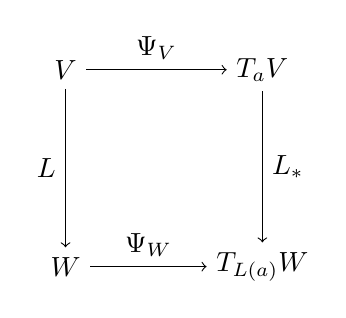
\begin{tikzpicture}[node distance=2.5cm, auto]
			\node (V) {$V$};
			\node (TaV) [right of=V] {$T_a V$};
			\node (W) [below of=V] {$W$};
			\node (TaW) [right of=W] {$T_{L(a)} W$};
			
			\draw[->] (V) -- node {$\Psi_V$} (TaV);
			\draw[->] (V) -- node [left] {$L$} (W);
			\draw[->] (TaV) -- node [right] {$L_*$} (TaW);
			\draw[->] (W) -- node {$\Psi_W$} (TaW);
		\end{tikzpicture}
	\end{center}
}
\solucao{
	
	\textbf{Análise do Enunciado}
	\begin{itemize}
		\item \textbf{Hipóteses:} $V$ e $W$ são espaços vetoriais de dimensão finita; $a \in V$; $L : V \to W$ é uma aplicação linear.
		\item \textbf{Tese 1:} Construir um isomorfismo $\Psi_V : V \to T_a V$.
		\item \textbf{Tese 2:} Provar que $\Psi_W \circ L = L_* \circ \Psi_V$, ou seja, que o diagrama comutativo é válido.
	\end{itemize}
	
	\textbf{Fundamentação Teórica}
	Um espaço vetorial $V$ de dimensão $n$ é uma variedade suave com um atlas global composto por uma única carta $\varphi : V \to \mathbb{R}^n$ (qualquer isomorfismo de $V$ para $\mathbb{R}^n$ serve). 
	
	De acordo com a definição de Lee (Capítulo 3), o espaço tangente $T_a V$ consiste em todas as derivações em $a$. Para qualquer vetor $v \in V$, podemos definir uma derivação $\Psi_V(v) \in T_a V$ através da derivada direcional:
	\begin{equation*}
		(\Psi_V(v)) f = df_a(v) = \lim_{t \to 0} \frac{f(a + tv) - f(a)}{t}, \quad \forall f \in C^\infty(V).
	\end{equation*}
	A aplicação diferencial $L_* : T_a V \to T_{L(a)} W$ (push-forward) é definida por $(L_* X) h = X(h \circ L)$ para todo $X \in T_a V$ e $h \in C^\infty(W)$.
	
	\textbf{Desenvolvimento Formal}
	
	\textbf{1. Prova de que $\Psi_V$ é um isomorfismo:}
	A aplicação $\Psi_V : V \to T_a V$ é linear, pois o limite da soma é a soma dos limites e o limite do produto por escalar é o produto pelo escalar. 
	
	Para provar que $\Psi_V$ é um isomorfismo, observamos que $\dim(V) = n$ e, como $V$ é uma variedade suave de dimensão $n$, temos $\dim(T_a V) = n$. Portanto, basta provar que $\Psi_V$ é injetiva. 
	
	Suponha $\Psi_V(v) = 0$. Então, para toda função $f \in C^\infty(V)$, temos $df_a(v) = 0$. Escolhemos a função linear $f(x) = \ell(x)$ para algum $\ell \in V^*$ (o espaço dual de $V$). Para tal função, temos:
	\begin{equation*}
		df_a(v) = \lim_{t \to 0} \frac{\ell(a+tv) - \ell(a)}{t} = \lim_{t \to 0} \frac{\ell(a) + t\ell(v) - \ell(a)}{t} = \ell(v).
	\end{equation*}
	Como $\ell(v) = 0$ para toda $\ell \in V^*$, segue necessariamente que $v = 0$. Logo, $\Psi_V$ é injetiva e, consequentemente, um isomorfismo.
	
	\textbf{2. Prova da Comutatividade do Diagrama:}
	Desejamos mostrar que $\Psi_W \circ L = L_* \circ \Psi_V$. Seja $v \in V$. Aplicamos ambas as composições a uma função arbitrária $h \in C^\infty(W)$.
	
	Primeiro, calculamos a ação de $\Psi_W(L(v))$ sobre $h$:
	\begin{equation*}
		(\Psi_W(L(v))) h = dh_{L(a)}(L(v)) = \lim_{t \to 0} \frac{h(L(a) + tL(v)) - h(L(a))}{t}.
	\end{equation*}
	Como $L$ é linear, temos $L(a) + tL(v) = L(a + tv)$. Assim:
	\begin{equation*}
		(\Psi_W(L(v))) h = \lim_{t \to 0} \frac{h(L(a + tv)) - h(L(a))}{t}.
	\end{equation*}
	
	Agora, calculamos a ação de $L_* (\Psi_V(v))$ sobre $h$:
	\begin{align*}
		(L_* (\Psi_V(v))) h &= (\Psi_V(v))(h \circ L) \quad (\text{pela definição de } L_*) \\
		&= d(h \circ L)_a(v) \quad (\text{pela definição de } \Psi_V) \\
		&= \lim_{t \to 0} \frac{(h \circ L)(a + tv) - (h \circ L)(a)}{t} \\
		&= \lim_{t \to 0} \frac{h(L(a + tv)) - h(L(a))}{t}.
	\end{align*}
	
	Comparando os dois resultados, vemos que:
	\begin{equation*}
		(\Psi_W \circ L)(v) = (L_* \circ \Psi_V)(v).
	\end{equation*}
	Como isso é válido para todo $v \in V$, a aplicação $\Psi_W \circ L$ é igual a $L_* \circ \Psi_V$. Portanto, o diagrama comuta.
}
%%%% QUESTÃO 09 %%%%
\questao{
	Sejam $M^{n}$ e $N^{k}$ variedades suaves, com $M^{n}$ conexa, e $F : M^{n} \to N^{k}$ uma aplicação suave tal que $F_* : T_p M \to T_{F(p)} N$ é a aplicação nula, para todo $p \in M^{n}$. Mostre que $F$ é constante.
}
\solucao{
	
	\textbf{Análise do Enunciado}
	\begin{itemize}
		\item \textbf{Hipóteses:} $M^n$ é uma variedade suave e conexa; $N^k$ é uma variedade suave; $F : M^n \to N^k$ é suave; para todo $p \in M^n$, o diferencial $F_{*,p}$ é o operador nulo ($F_{*,p}(v) = 0$ para todo $v \in T_p M$).
		\item \textbf{Tese:} Provar que $F(p) = F(q)$ para quaisquer $p, q \in M^n$.
	\end{itemize}
	
	\textbf{Fundamentação Teórica}
	Para a demonstração, utilizaremos os seguintes conceitos e resultados:
	\begin{enumerate}
		\item \textbf{Conexidade por Caminhos:} Como demonstrado na \textbf{Questão 02 da Lista 01}, para uma variedade suave, a conexidade topológica é equivalente à conexidade por caminhos. Assim, a hipótese de que $M^n$ é conexa garante que, para quaisquer $p, q \in M^n$, existe uma curva suave $\gamma : [0, 1] \to M^n$ tal que $\gamma(0) = p$ e $\gamma(1) = q$.
		\item \textbf{Regra da Cadeia:} Se $\gamma : [0, 1] \to M^n$ é uma curva suave, a derivada de $\gamma$ no tempo $t$ é um vetor tangente $\gamma'(t) \in T_{\gamma(t)} M$. A aplicação composta $F \circ \gamma : [0, 1] \to N^k$ é uma curva suave em $N^k$ cujo vetor tangente é dado por:
		\begin{equation*}
			(F \circ \gamma)'(t) = F_*(\gamma'(t)).
		\end{equation*}
		\item \textbf{Teorema do Valor Médio (ou Fundamental do Cálculo):} Em $\mathbb{R}^k$, se a derivada de uma função é nula em todo o intervalo, a função é constante.
	\end{enumerate}
	
	\textbf{Desenvolvimento Formal}
	
	Sejam $p, q$ dois pontos quaisquer em $M^n$. Pelo resultado citado anteriormente, existe uma curva suave $\gamma : [0, 1] \to M^n$ tal que $\gamma(0) = p$ e $\gamma(1) = q$. Consideremos a aplicação composta:
	\begin{equation*}
		\sigma : [0, 1] \to N^k, \quad \sigma(t) = (F \circ \gamma)(t).
	\end{equation*}
	A aplicação $\sigma$ é uma curva suave em $N^k$. Para analisar o comportamento de $\sigma$, escolhemos um atlas suave para $N^k$. Para cada $t \in [0, 1]$, seja $(V, \psi)$ uma carta coordenada em $N^k$ tal que $\sigma(t) \in V$. A representação coordenada da curva, $\hat{\sigma} = \psi \circ \sigma$, é uma aplicação de um intervalo para $\mathbb{R}^k$.
	
	A derivada de $\hat{\sigma}$ no tempo $t$ é dada por:
	\begin{align*}
		\frac{d}{dt} (\psi \circ F \circ \gamma)(t) &= d\psi_{\sigma(t)} \left( (F \circ \gamma)'(t) \right) \\
		&= d\psi_{\sigma(t)} \left( F_*(\gamma'(t)) \right).
	\end{align*}
	Por hipótese, o diferencial $F_*$ é a aplicação nula para todo ponto de $M^n$. Como $\gamma'(t) \in T_{\gamma(t)} M$, temos que $F_*(\gamma'(t)) = 0$ para todo $t \in [0, 1]$. Substituindo na expressão anterior:
	\begin{equation*}
		\frac{d}{dt} (\psi \circ F \circ \gamma)(t) = d\psi_{\sigma(t)}(0) = 0.
	\end{equation*}
	Sendo a derivada de $\hat{\sigma}$ nula para todo $t$ em seu domínio, a função $\hat{\sigma}$ é constante em cada componente do intervalo $[0,1]$. Como a representação coordenada é constante e $\psi$ é um homeomorfismo, a curva $\sigma(t)$ é constante em $N^k$.
	
	Portanto, temos que:
	\begin{equation*}
		\sigma(0) = \sigma(1) \implies F(\gamma(0)) = F(\gamma(1)) \implies F(p) = F(q).
	\end{equation*}
	Como $p$ e $q$ foram escolhidos arbitrariamente em $M^n$, concluímos que $F$ assume um único valor em todo o domínio. Logo, $F$ é constante.
}
%%%% QUESTÃO 10 %%%%
\questao{
	Mostre que se uma $n$-variedade suave (não vazia) é difeomorfa a uma $k$-variedade suave, então $n = k$.
}
\solucao{
	
	\textbf{Análise do Enunciado}
	\begin{itemize}
		\item \textbf{Hipóteses:} $M^n$ e $N^k$ são variedades suaves não vazias e existe um difeomorfismo $f : M^n \to N^k$.
		\item \textbf{Tese:} Provar que as dimensões são iguais, ou seja, $n = k$.
	\end{itemize}
	
	\textbf{Fundamentação Teórica}
	Um difeomorfismo $f : M^n \to N^k$ é, por definição, uma aplicação suave que possui uma inversa suave $f^{-1}$. Consequentemente, $f$ é, em particular, um \textbf{difeomorfismo local} em cada ponto $p \in M^n$.
	
	Utilizaremos o resultado obtido na \textbf{Questão 07 desta Lista 02}, que estabelece que, se $f$ é um difeomorfismo local, então a aplicação diferencial $f_* : T_p M \to T_{f(p)} N$ é um isomorfismo de espaços vetoriais para todo $p \in M^n$.
	
	\textbf{Desenvolvimento Formal}
	
	Seja $f : M^n \to N^k$ um difeomorfismo. Fixemos um ponto $p \in M^n$. Como $f$ é um difeomorfismo, ele é um difeomorfismo local em $p$. Pelo resultado da \textbf{Questão 07}, a aplicação diferencial:
	\begin{equation*}
		f_* : T_p M \longrightarrow T_{f(p)} N
	\end{equation*}
	é um isomorfismo de espaços vetoriais. 
	
	De acordo com a teoria fundamental de álgebra linear, dois espaços vetoriais são isomorfos se, e somente se, possuem a mesma dimensão. Sabemos que:
	\begin{enumerate}
		\item A dimensão do espaço tangente $T_p M$ é igual à dimensão da variedade $M$, logo $\dim(T_p M) = n$.
		\item A dimensão do espaço tangente $T_{f(p)} N$ é igual à dimensão da variedade $N$, logo $\dim(T_{f(p)} N) = k$.
	\end{enumerate}
	
	Sendo $f_*$ um isomorfismo, segue necessariamente que:
	\begin{equation*}
		\dim(T_p M) = \dim(T_{f(p)} N) \implies n = k.
	\end{equation*}
	Dessa forma, a dimensão de uma variedade suave é um invariante sob difeomorfismos.
}
%%%% QUESTÃO 11 %%%%
\questao{
	Mostre que a aplicação $F : \mathbb{R}^3 \to \mathbb{R}^6$ definida por $$F(x, y, z) = (x^2, y^2, z^2, \sqrt{2}xy, \sqrt{2}xz, \sqrt{2}yz),$$ induz uma aplicação suave injetiva $f : \mathbb{RP}^2 \to \mathbb{S}^5$ cuja derivada $Df$ também é injetiva.
}
\solucao{
	\textbf{Análise do Enunciado}
	\begin{itemize}
		\item \textbf{Hipóteses:} $F$ é a aplicação polinomial dada de $\mathbb{R}^3$ para $\mathbb{R}^6$.
		\item \textbf{Tese 1:} $F$ induz uma aplicação suave $f: \mathbb{RP}^2 \to \mathbb{S}^5$.
		\item \textbf{Tese 2:} A aplicação $f$ é injetiva.
		\item \textbf{Tese 3:} A derivada (diferencial) $Df$ é injetiva em cada ponto (ou seja, $f$ é uma imersão).
	\end{itemize}
	
	\textbf{Fundamentação Teórica}
	Conforme demonstrado nas \textbf{Questões 19 e 20 da Lista 01}, a aplicação $F$ satisfaz $F(\mathbb{S}^2) \subset \mathbb{S}^5$ e $F(x) = F(-x)$ para todo $x \in \mathbb{S}^2$. Pela teoria de variedades quocientes, isso garante a existência de uma aplicação suave $\bar{f} : \mathbb{RP}^2 \to \mathbb{S}^5$ tal que $F|_{\mathbb{S}^2} = \bar{f} \circ \pi$, onde $\pi : \mathbb{S}^2 \to \mathbb{RP}^2$ é a projeção canônica.
	
	A injetividade de $f$ foi rigorosamente provada na \textbf{Questão 27 da Lista 01}, onde se demonstrou que $$F(x) = F(y) \implies x = \pm ,y$$ o que implica $[x] = [y]$ em $\mathbb{RP}^2$.
	
	Para a injetividade de $Df$, utilizaremos a caracterização do espaço tangente à esfera. Na \textbf{Questão 3(b) da Lista 01}, definimos $\mathbb{S}^2$ como o conjunto nível $f^{-1}(1)$ de $f(x) = |x|^2$. Pelo Teorema do Valor Regular, o espaço tangente $T_p \mathbb{S}^2$ é o núcleo do diferencial $df_p$. Como $\nabla f(p) = 2p$, temos que um vetor $v \in \mathbb{R}^3$ pertence a $T_p \mathbb{S}^2$ se, e somente se:
	\begin{equation*}
		df_p(v) = \langle \nabla f(p), v \rangle = \langle 2p, v \rangle = 0 \iff \langle p, v \rangle = 0.
	\end{equation*}
	Assim, $T_p \mathbb{S}^2$ é o hiperplano ortogonal ao vetor posição $p$.
	
	\textbf{Desenvolvimento Formal}
	
	\textbf{1. Indução e Injetividade de $f$:}
	As teses de que $f$ está bem definida, é suave e é injetiva seguem diretamente dos resultados obtidos nas \textbf{Questões 19, 20 e 27 da Lista 01}.
	
	\textbf{2. Injetividade da Derivada $Df$:}
	Para provar que $df_{[x]}$ é injetivo, analisamos o diferencial de $F$ em um ponto $p = (x, y, z) \in \mathbb{S}^2$. O diferencial $DF_p$ é representado pela matriz Jacobiana de $F$:
	\begin{equation*}
		DF_p = \begin{bmatrix} 
			2x & 0 & 0 \\ 
			0 & 2y & 0 \\ 
			0 & 0 & 2z \\ 
			\sqrt{2}y & \sqrt{2}x & 0 \\ 
			\sqrt{2}z & 0 & \sqrt{2}x \\ 
			0 & \sqrt{2}z & \sqrt{2}y 
		\end{bmatrix}.
	\end{equation*}
	Seja $v = (v_1, v_2, v_3) \in T_p \mathbb{S}^2$. Pela fundamentação acima, temos a restrição $\langle p, v \rangle = xv_1 + yv_2 + zv_3 = 0$.
	
	Suponhamos que $DF_p(v) = 0$. Isso implica que todas as componentes do vetor resultante sejam nulas:
	\begin{align*}
		2xv_1 = 0, \quad 2yv_2 = 0, \quad 2zv_3 = 0, \quad \sqrt{2}(yv_1 + xv_2) = 0, \quad \sqrt{2}(zv_1 + xv_3) = 0, \quad \text{e} \quad \sqrt{2}(zv_2 + yv_3) = 0.
	\end{align*}
	
	Analisamos a consistência desse sistema:
	\begin{enumerate}
		\item Se $x, y, z \neq 0$, as três primeiras equações implicam imediatamente que $v_1 = v_2 = v_3 = 0$, logo $v = 0$.
		\item Se alguma coordenada for nula, por exemplo, $x = 0$, então $p = (0, y, z)$ com $y^2 + z^2 = 1$. As equações tornam-se:
		\begin{equation*}
			0 = 0, \quad 2yv_2 = 0, \quad 2zv_3 = 0, \quad \sqrt{2}yv_1 = 0, \quad \sqrt{2}zv_1 = 0, \quad \sqrt{2}(zv_2 + yv_3) = 0.
		\end{equation*}
		Como $y$ e $z$ não podem ser ambos nulos, a quarta e quinta equações ($\sqrt{2}yv_1 = 0$ e $\sqrt{2}zv_1 = 0$) forçam $v_1 = 0$. 
		
		As equações $2yv_2 = 0$ e $2zv_3 = 0$ forçam $v_2 = 0$ e $v_3 = 0$ respectivamente (pois se $y=0$, então $z \neq 0$ e vice-versa).
	\end{enumerate}
	Em todos os casos, $DF_p(v) = 0 \implies v = 0$ para qualquer $v \in T_p \mathbb{S}^2$. Assim, o diferencial $DF_p$ é injetivo quando restrito ao espaço tangente da esfera.
	
	Como $F|_{\mathbb{S}^2} = f \circ \pi$, pela regra da cadeia temos $(F|_{\mathbb{S}^2})_* = f_* \circ \pi_*$. Visto que $\pi_*$ é um isomorfismo (pois é difeomorfismo local), a injetividade de $(F|_{\mathbb{S}^2})_*$ implica a injetividade de $f_*$ (ou $Df$).
}
%%%% QUESTÃO 12 %%%%
\questao{
	Mostre que a aplicação $F : \mathbb{R}^3 \to \mathbb{R}^5$ definida por 
	$$F(x, y, z) = \left(\sqrt{3}xy, \sqrt{3}xz, \sqrt{3}yz, \frac{\sqrt{3}}{2}(x^2 - y^2), \frac{1}{2}x^2 + \frac{1}{2}y^2 - z^2\right),$$ 
	induz uma aplicação suave injetiva $\bar{f} : \mathbb{RP}^2 \to \mathbb{S}^4$ cuja derivada $D\bar{f}$ também é injetiva.
}
\solucao{
	
	\textbf{Análise do Enunciado}
	\begin{itemize}
		\item \textbf{Hipóteses:} $F$ é uma aplicação polinomial de $\mathbb{R}^3$ para $\mathbb{R}^5$.
		\item \textbf{Tese 1:} Provar que $F$ induz uma aplicação $\bar{f} : \mathbb{RP}^2 \to \mathbb{S}^4$ bem definida e suave.
		\item \textbf{Tese 2:} Provar que $\bar{f}$ é injetiva.
		\item \textbf{Tese 3:} Provar que a derivada $D\bar{f}$ é injetiva em cada ponto (ou seja, $\bar{f}$ é uma imersão).
	\end{itemize}
	
	\textbf{Fundamentação Teórica}
	\begin{enumerate}
		\item \textbf{Mapas Induzidos em Espaços Projetivos:} De acordo com a teoria de variedades quocientes (Lee, Cap. 4), uma aplicação $F: \mathbb{R}^{n+1}\setminus\{0\} \to \mathbb{R}^{m+1}\setminus\{0\}$ induz um mapa suave $\bar{f}: \mathbb{RP}^n \to \mathbb{RP}^m$ se, e somente se, $F$ for constante nas fibras da projeção $\pi$, o que é garantido se $F$ for homogênea de algum grau $d$. Este princípio foi aplicado na \textbf{Questão 28 da Lista 01}.
		\item \textbf{Subvariedades e a Esfera $\mathbb{S}^n$:} Para que a imagem de $\bar{f}$ esteja em $\mathbb{S}^4$, devemos provar que a norma euclidiana $\|F(p)\|$ é unitária para todo $p \in \mathbb{S}^2$.
		\item \textbf{Injetividade e a Relação de Equivalência:} A injetividade de $\bar{f}$ requer que $F(x) = F(y) \implies x = \pm y$. A lógica de resolução de sistemas de equações quadráticas para este fim foi estabelecida na \textbf{Questão 27 da Lista 01}.
		\item \textbf{Imersões e o Diferencial:} Uma aplicação suave $f: M \to N$ é uma imersão se seu diferencial $df_p: T_p M \to T_{f(p)} N$ for injetivo para todo $p \in M$. Para $M = \mathbb{S}^2$, o espaço tangente $T_p \mathbb{S}^2$ é caracterizado por $\{v \in \mathbb{R}^3 : \langle p, v \rangle = 0\}$ (Lee, Cap. 3; \textbf{Questão 3b da Lista 01}).
	\end{enumerate}
	
	\textbf{Desenvolvimento Formal}
	
	\textbf{1. Indução e Suavidade da Aplicação $\bar{f}$}
	
	Seja $p = (x, y, z) \in \mathbb{S}^2$. Note que $F$ é homogênea de grau 2, pois para qualquer $\lambda \in \mathbb{R}\setminus\{0\}$:
	\begin{align*}
		F(\lambda x, \lambda y, \lambda z) &= \left(\sqrt{3}\lambda^2 xy, \sqrt{3}\lambda^2 xz, \sqrt{3}\lambda^2 yz, \frac{\sqrt{3}}{2}(\lambda^2 x^2 - \lambda^2 y^2), \frac{1}{2}\lambda^2 x^2 + \frac{1}{2}\lambda^2 y^2 - \lambda^2 z^2\right) \\
		&= \lambda^2 F(x, y, z).
	\end{align*}
	Pela fundamentação citada, $F$ induz um mapa $\bar{f}: \mathbb{RP}^2 \to \mathbb{RP}^4$ dado por $\bar{f}([p]) = [F(p)]$. Como $\|F(p)\|^2 = 1$ para $p \in \mathbb{S}^2$ (verificação abaixo), a imagem de cada classe $[p]$ pode ser representada por um único vetor unitário em $\mathbb{S}^4$, permitindo a definição $\bar{f}: \mathbb{RP}^2 \to \mathbb{S}^4$.
	
	Verificação da norma para $p \in \mathbb{S}^2$ ($x^2+y^2+z^2=1$):
	\begin{align*}
		\|F(p)\|^2 &= 3(x^2y^2 + x^2z^2 + y^2z^2) + \frac{3}{4}(x^4 + y^4 - 2x^2y^2) + \left(\frac{1}{4}x^4 + \frac{1}{4}y^4 + z^4 + \frac{1}{2}x^2y^2 - x^2z^2 - y^2z^2\right) \\
		&= x^4 + y^4 + z^4 + 2x^2y^2 + 2x^2z^2 + 2y^2z^2 = (x^2 + y^2 + z^2)^2 = 1.
	\end{align*}
	
	\textbf{2. Prova de Injetividade}
	
	Sejam $[x], [y] \in \mathbb{RP}^2$ tais que $\bar{f}([x]) = \bar{f}([y])$. Para representantes $x, y \in \mathbb{S}^2$, temos $F(x) = F(y)$, resultando no sistema:
	\begin{enumerate}[label=(\roman*)]
		\item $x_1x_2 = y_1y_2$; (ii) $x_1x_3 = y_1y_3$; (iii) $x_2x_3 = y_2y_3$; (iv) $x_1^2 - x_2^2 = y_1^2 - y_2^2$; (v) $\frac{1}{2}x_1^2 + \frac{1}{2}x_2^2 - x_3^2 = \frac{1}{2}y_1^2 + \frac{1}{2}y_2^2 - y_3^2$.
	\end{enumerate}
	Da equação (v), e utilizando $x_1^2+x_2^2 = 1-x_3^2$, temos:
	\begin{align*}
		\frac{1}{2}(1-x_3^2) - x_3^2 &= \frac{1}{2}(1-y_3^2) - y_3^2 \implies \frac{1}{2} - \frac{3}{2}x_3^2 = \frac{1}{2} - \frac{3}{2}y_3^2 \implies x_3^2 = y_3^2.
	\end{align*}
	Combinando $x_1^2+x_2^2 = y_1^2+y_2^2$ com a equação (iv) ($x_1^2-x_2^2 = y_1^2-y_2^2$), obtemos por soma e subtração:
	\begin{align*}
		2x_1^2 = 2y_1^2 \implies x_1^2 = y_1^2 \quad \text{e} \quad 2x_2^2 = 2y_2^2 \implies x_2^2 = y_2^2.
	\end{align*}
	Como $x_i^2 = y_i^2$ e $x_ix_j = y_iy_j$, a lógica da \textbf{Questão 27 da Lista 01} implica que $y = \pm x$. Logo, $[x] = [y]$.
	
	\textbf{3. Injetividade da Derivada $D\bar{f}$}
	
	A matriz Jacobiana $DF_p$ é:
	\begin{equation*}
		DF_p = \begin{bmatrix} 
			\sqrt{3}y & \sqrt{3}x & 0 \\ \sqrt{3}z & 0 & \sqrt{3}x \\ 0 & \sqrt{3}z & \sqrt{3}y \\ \sqrt{3}x & -\sqrt{3}y & 0 \\ x & y & -2z 
		\end{bmatrix}.
	\end{equation*}
	Seja $v \in T_p\mathbb{S}^2$, logo $xv_1 + yv_2 + zv_3 = 0$. Suponhamos $DF_p(v) = 0$:
	\begin{align*}
		\sqrt{3}(yv_1 + xv_2) &= 0 \quad (1) \\
		\sqrt{3}(xv_1 - yv_2) &= 0 \quad (2) \\
		\sqrt{3}(zv_1 + xv_3) &= 0 \quad (3)
	\end{align*}
	Das equações (1) e (2), o determinante do sistema em $v_1, v_2$ é $-(y^2+x^2)$. 
	Se $x^2+y^2 \neq 0$, então $v_1=v_2=0$, e por $\langle p, v \rangle = 0$, temos $zv_3=0 \implies v_3=0$.
	Se $x^2+y^2=0$, então $x=0, y=0 \implies z=\pm 1$. A condição $\langle p, v \rangle = 0$ implica $v_3=0$. Substituindo na Jacobiana, a linha 2 dá $\pm\sqrt{3}v_1=0$ e a linha 3 dá $\pm\sqrt{3}v_2=0$. 
	Em todos os casos, $v=0$. O núcleo de $DF_p|_{T_p\mathbb{S}^2}$ é trivial. Como $\pi_*$ é um isomorfismo, a derivada $D\bar{f}$ é injetiva.
}
%%%% QUESTÃO 13 %%%%
\questao{
	Seja $M^n$ uma $n$-variedade suave. Mostre que o fibrado tangente $TM$ admite uma topologia e uma estrutura suave de tal forma que $TM$ é uma $2n$-variedade suave.
}
\solucao{
	
	\textbf{Análise do Enunciado}
	\begin{itemize}
		\item \textbf{Hipóteses:} $M^n$ é uma $n$-variedade suave.
		\item \textbf{Tese:} Provar que o conjunto $TM = \bigcup_{p \in M} T_p M$ possui uma topologia e um atlas suave que o tornam uma variedade suave de dimensão $2n$.
	\end{itemize}
	
	\textbf{Fundamentação Teórica}
	\begin{enumerate}
		\item \textbf{Definição do Espaço Tangente:} Como estabelecido na \textbf{Lista 01}, para cada $p \in M$, $T_p M$ é um espaço vetorial de dimensão $n$. O fibrado tangente $TM$ é a união disjunta de todos esses espaços.
		\item \textbf{Construção de Atlas Induzidos:} Se $\mathcal{U} = \{(U_\alpha, \phi_\alpha)\}_{\alpha \in \Lambda}$ é um atlas suave para $M$, podemos definir a \textbf{extensão} desse atlas para $TM$. Para cada $\alpha \in \Lambda$, definimos o conjunto $T U_\alpha = \bigcup_{p \in U_\alpha} T_p M$, que é um subconjunto de $TM$.
		\item \textbf{Mapeamentos de Coordenadas:} A aplicação $\Phi_\alpha : T U_\alpha \to \mathbb{R}^{2n}$ é definida enviando um vetor $(p, v)$ para a coordenada do ponto $p$ e para as componentes do vetor $v$ na base induzida pela carta $\phi_\alpha$.
		\item \textbf{Axiomas de Variedade:} Para que $TM$ seja uma variedade, devemos garantir que a topologia induzida seja de Hausdorff, possua base enumerável e que as funções de transição sejam $C^\infty$.
	\end{enumerate}
	
	\textbf{Desenvolvimento Formal}
	
	\textbf{1. Definição das Cartas de $TM$}
	
	Seja $\phi_\alpha : U_\alpha \to \mathbb{R}^n$ uma carta de $M$. Para qualquer $p \in U_\alpha$, o diferencial da carta no ponto $p$ é uma aplicação linear:
	\begin{equation*}
		d(\phi_\alpha)_p : T_p M \to T_{\phi_\alpha(p)} \mathbb{R}^n \cong \mathbb{R}^n.
	\end{equation*}
	Como $\phi_\alpha$ é um homeomorfismo, $d(\phi_\alpha)_p$ é um isomorfismo de espaços vetoriais. Definimos a aplicação $\Phi_\alpha : T U_\alpha \to \mathbb{R}^{2n}$ por:
	\begin{equation*}
		\Phi_\alpha(p, v) = (\phi_\alpha(p), d(\phi_\alpha)_p(v)).
	\end{equation*}
	Seja $u = \phi_\alpha(p) \in \mathbb{R}^n$ e $\xi = d(\phi_\alpha)_p(v) \in \mathbb{R}^n$. A inversa $\Phi_\alpha^{-1} : \phi_\alpha(U_\alpha) \times \mathbb{R}^n \to T U_\alpha$ é dada por:
	\begin{equation*}
		\Phi_\alpha^{-1}(u, \xi) = (\phi_\alpha^{-1}(u), \sum_{i=1}^n \xi^i \frac{\partial}{\partial x^i} \Big|_{\phi_\alpha^{-1}(u)}).
	\end{equation*}
	
	\textbf{2. Construção da Topologia}
	
	Definimos a topologia em $TM$ declarando que um conjunto $W \subset TM$ é aberto se, e somente se, $\Phi_\alpha(W \cap T U_\alpha)$ é um aberto de $\mathbb{R}^{2n}$ para cada $\alpha \in \Lambda$. 
	
	Como as cartas $\Phi_\alpha$ são homeomorfismos sobre abertos de $\mathbb{R}^{2n}$, e $M$ é de Hausdorff e possui base enumerável, as mesmas propriedades são herdadas por $TM$. De fato, se $p, q \in M$ são distintos, eles podem ser separados em $M$, e consequentemente seus fibrados tangentes podem ser separados em $TM$. Se $\mathcal{B}$ é uma base enumerável para $M$, então $\mathcal{B} \times \mathbb{Q}^n$ (ou qualquer base enumerável de $\mathbb{R}^n$) induz uma base enumerável para $TM$.
	
	\textbf{3. Suavidade das Funções de Transição}
	
	Sejam $(U_\alpha, \phi_\alpha)$ e $(U_\beta, \phi_\beta)$ duas cartas de $M$ com $U_\alpha \cap U_\beta \neq \emptyset$. A função de transição na base $M$ é $$\tau = \phi_\beta \circ \phi_\alpha^{-1} : \phi_\alpha(U_\alpha \cap U_\beta) \to \phi_\beta(U_\alpha \cap U_\beta).$$
	
	A função de transição em $TM$ é $\Psi = \Phi_\beta \circ \Phi_\alpha^{-1}$. Para $(u, \xi) \in \mathbb{R}^n \times \mathbb{R}^n$:
	\begin{align*}
		\Psi(u, \xi) &= \Phi_\beta(\Phi_\alpha^{-1}(u, \xi)) \\
		&= \Phi_\beta(p, v) \quad \text{onde } p = \phi_\alpha^{-1}(u) \text{ e } v = \sum \xi^i \frac{\partial}{\partial x^i} \Big|_p \\
		&= (\phi_\beta(p), d(\phi_\beta)_p(v)) \\
		&= (\phi_\beta(\phi_\alpha^{-1}(u)), d(\phi_\beta)_p(d(\phi_\alpha)^{-1}_p(\xi))).
	\end{align*}
	Pela regra da cadeia para diferenciais, temos $d(\phi_\beta)_p \circ d(\phi_\alpha)^{-1}_p = d(\phi_\beta \circ \phi_\alpha^{-1})_{\phi_\alpha(p)}$. Portanto:
	\begin{equation*}
		\Psi(u, \xi) = (\tau(u), d\tau_u(\xi)).
	\end{equation*}
	Como $M$ é uma variedade suave, $\tau$ é uma aplicação $C^\infty$. O diferencial $d\tau_u$ é representado pela matriz Jacobiana $J_\tau(u)$, cujas entradas são as derivadas parciais de $\tau$. Como $\tau$ é $C^\infty$, suas derivadas parciais também são $C^\infty$. 
	
	Logo, a aplicação $(u, \xi) \mapsto (\tau(u), J_\tau(u) \cdot \xi)$ é a composição de funções suaves em $\mathbb{R}^{2n}$, sendo, portanto, suave.
	
	\textbf{Conclusão}
	
	Tendo definido um atlas $\mathcal{T} = \{(T U_\alpha, \Phi_\alpha)\}$ com funções de transição suaves, e tendo verificado as propriedades topológicas de Hausdorff e base enumerável, concluímos que $TM$ é uma variedade suave de dimensão $n + n = 2n$.
}
%%%% RESULTADO EXTRA %%%%
Abaixo, estabelecemos um resultado fundamental da teoria de Grupos de Lie. Este teorema demonstra que a estrutura algébrica de um grupo, quando compatível com a estrutura de variedade suave, impõe uma rigidez geométrica ao fibrado tangente, tornando-o globalmente trivial. Este resultado será utilizado como base para as \textbf{Soluções Alternativas} das Questões 14 e 15, permitindo que a prova de trivialidade do fibrado tangente seja reduzida a uma propriedade de simetria do grupo.

\resultadoextra{Trivialidade do Fibrado Tangente de Grupos de Lie}{
	Seja $G$ um Grupo de Lie de dimensão $n$. Então $TG$ é difeomorfo a $G \times \mathbb{R}^n$.
}
\solucao{

	Seja $e \in G$ o elemento neutro do grupo. Para cada $g \in G$, definimos a aplicação de translação à esquerda $L_g : G \to G$ por $L_g(h) = gh$. Por definição de Grupo de Lie, a multiplicação é suave, logo $L_g$ é uma aplicação suave. Como $L_g$ possui inversa suave $L_{g^{-1}}$, então $L_g$ é um difeomorfismo de $G$ em si mesmo.
	
	O diferencial de $L_g$ no ponto $e$, denotado por $(L_g)_* : T_e G \to T_g G$, é um isomorfismo de espaços vetoriais, pois é o diferencial de um difeomorfismo. 
	
	Definimos a aplicação $\Psi : G \times T_e G \to TG$ por:
	\begin{equation*}
		\Psi(g, v) = (g, (L_g)_* v).
	\end{equation*}
	
	\textbf{1. Bijetividade:} Para qualquer vetor tangente $(p, w) \in TG$, onde $p \in G$ e $w \in T_p G$, existe um único $v \in T_e G$ tal que $(L_p)_* v = w$, dado que $v = (L_{p^{-1}})_* w$. Assim, $\Psi(p, v) = (p, w)$, provando que $\Psi$ é bijetiva.
	
	\textbf{2. Suavidade:} A suavidade de $\Psi$ decorre da suavidade da operação de multiplicação do grupo. Em coordenadas locais, a aplicação $(g, v) \mapsto (L_g)_* v$ é representada por funções suaves nas entradas de $g$ e $v$.
	
	\textbf{3. Suavidade da Inversa:} A inversa $\Psi^{-1} : TG \to G \times T_e G$ é dada por:
	\begin{equation*}
		\Psi^{-1}(p, w) = (p, (L_{p^{-1}})_* w).
	\end{equation*}
	Visto que a inversão $p \mapsto p^{-1}$ e a translação são suaves, $\Psi^{-1}$ também é suave.
	
	Como $T_e G$ é um espaço vetorial de dimensão $n$, ele é isomorfo a $\mathbb{R}^n$. Logo, temos o difeomorfismo $TG \cong G \times \mathbb{R}^n$.
}
%%%% QUESTÃO 14 %%%%
\questao{
	Mostre que $T\mathbb{R}^n$ é difeomorfo a $\mathbb{R}^{2n}$.
}
\solucao{
	
	\textbf{Análise do Enunciado}
	\begin{itemize}
		\item \textbf{Hipóteses:} O espaço base é a variedade suave $\mathbb{R}^n$.
		\item \textbf{Tese:} Provar a existência de um difeomorfismo entre o fibrado tangente $T\mathbb{R}^n$ e o espaço euclidiano $\mathbb{R}^{2n}$.
	\end{itemize}
	
	\textbf{Fundamentação Teórica}
	Utilizamos a construção de atlas induzidos para o fibrado tangente (Lee, Cap. 3). Para uma variedade que admite uma carta global $(M, \phi)$, o fibrado tangente é trivializado pela aplicação $\Phi(p, v) = (\phi(p), d\phi_p(v))$.
	
	\textbf{Desenvolvimento Formal}
	
	Seja $\phi = \text{Id}_{\mathbb{R}^n}$ a carta global para $\mathbb{R}^n$. Para qualquer ponto $p \in \mathbb{R}^n$, o diferencial da identidade $$d(\text{Id}_{\mathbb{R}^n})_p : T_p\mathbb{R}^n \to T_p\mathbb{R}^n \cong \mathbb{R}^n $$ é a aplicação identidade nos espaços tangentes. Definimos $\Psi : T\mathbb{R}^n \to \mathbb{R}^{2n}$ por:
	\begin{equation*}
		\Psi(p, v) = (p, v).
	\end{equation*}
	Onde $v$ é representado por suas componentes na base canônica $\left\{\frac{\partial}{\partial x^i}\right\}$.
	
	\textbf{1. Bijetividade:} Para qualquer par $(u, \xi) \in \mathbb{R}^n \times \mathbb{R}^n$, existe um único ponto $p = u \in \mathbb{R}^n$ e um único vetor $v = \sum_{i=1}^n \xi^i \frac{\partial}{\partial x^i} \Big|_p \in T_p\mathbb{R}^n$ tal que $\Psi(p, v) = (u, \xi)$. Logo, $\Psi$ é bijetiva.
	
	\textbf{2. Suavidade de $\Psi$ e $\Psi^{-1}$:}
	A aplicação $\Psi$ é, por construção, a própria carta $\Phi$ definida na Questão 13 para a identidade. Como a função de transição para uma única carta é a identidade $\text{Id}_{\mathbb{R}^{2n}}$, que é infinitamente diferenciável, $\Psi$ é suave.
	
	A inversa $\Psi^{-1} : \mathbb{R}^{2n} \to T\mathbb{R}^n$ é dada por:
	\begin{equation*}
		\Psi^{-1}(u, \xi) = \left( u, \sum_{i=1}^n \xi^i \frac{\partial}{\partial x^i} \Big|_u \right).
	\end{equation*}
	Sendo $\Psi^{-1}$ a inversa de um homeomorfismo que define a estrutura suave de $T\mathbb{R}^n$, ela é, por definição, suave.
	
	\textbf{Conclusão}
	Como $\Psi$ é uma bijecção suave com inversa suave, ela é um difeomorfismo. Portanto, $T\mathbb{R}^n \cong \mathbb{R}^{2n}$.
}
\solucaoalt{
	
	\textbf{Análise via Grupos de Lie}
	
	Como provamos na \textbf{Questão 36(a) da Lista 01}, $\mathbb{R}^n$ é um Grupo de Lie sob a operação de adição usual. 
	
	De acordo com o resultado extra demonstrado anteriormente, o fibrado tangente de qualquer Grupo de Lie $G$ é trivial, sendo difeomorfo a $G \times T_e G$. No caso de $\mathbb{R}^n$, o elemento neutro é o vetor nulo $0$. A translação à esquerda $L_g: \mathbb{R}^n \to \mathbb{R}^n$ é dada por $L_g(h) = g+h$.
	
	O diferencial $(L_g)_* : T_0\mathbb{R}^n \to T_g\mathbb{R}^n$ é um isomorfismo. Definimos a aplicação:
	\begin{equation*}
		\Psi : \mathbb{R}^n \times T_0\mathbb{R}^n \to T\mathbb{R}^n, \quad \Psi(g, v) = (g, (L_g)_* v).
	\end{equation*}
	Visto que $T_0\mathbb{R}^n$ é um espaço vetorial de dimensão $n$, temos $T_0\mathbb{R}^n \cong \mathbb{R}^n$. Assim, $\Psi$ estabelece um difeomorfismo entre $\mathbb{R}^n \times \mathbb{R}^n$ e $T\mathbb{R}^n$. Como $\mathbb{R}^n \times \mathbb{R}^n$ é canonicamente difeomorfo a $\mathbb{R}^{2n}$, segue que $T\mathbb{R}^n \cong \mathbb{R}^{2n}$.
}
%%%% QUESTÃO 15 %%%%
\questao{
	Mostre que $T\mathbb{S}^1$ é difeomorfo a $\mathbb{S}^1 \times \mathbb{R}$.
}
\solucao{
	
	\textbf{Análise do Enunciado}
	\begin{itemize}
		\item \textbf{Hipóteses:} O espaço base é a 1-esfera $\mathbb{S}^1 \subset \mathbb{R}^2$.
		\item \textbf{Tese:} Provar que $T\mathbb{S}^1 \cong \mathbb{S}^1 \times \mathbb{R}$.
	\end{itemize}
	
	\textbf{Fundamentação Teórica}
	Uma variedade $M^n$ é paralelizável se admite $n$ campos de vetores suaves que formam uma base de $T_p M$ para todo $p \in M$. Se $M$ é paralelizável, então $TM \cong M \times \mathbb{R}^n$. Para $\mathbb{S}^1 \subset \mathbb{R}^2$, o espaço tangente em $p = (x, y)$ é $T_p\mathbb{S}^1 = \{v \in \mathbb{R}^2 : \langle p, v \rangle = 0\}$.
	
	\textbf{Desenvolvimento Formal}
	
	\textbf{1. Construção de um Campo de Vetores Global:}
	Definimos o campo de vetores $X$ em $\mathbb{S}^1$ por $X(p) = (-y, x)$ para $p=(x,y)$.
	\begin{itemize}
		\item \textbf{Tangencialidade:} $\langle p, X(p) \rangle = \langle (x, y), (-y, x) \rangle = -xy + yx = 0$. Logo, $X(p) \in T_p\mathbb{S}^1$.
		\item \textbf{Não-nulidade:} $\|X(p)\|^2 = (-y)^2 + x^2 = 1$. Logo, $X(p)$ nunca é nulo.
		\item \textbf{Suavidade:} As componentes são lineares, logo $X$ é suave.
	\end{itemize}
	Como $\dim(T_p\mathbb{S}^1)=1$ e $X(p) \neq 0$, o conjunto $\{X(p)\}$ é uma base de $T_p\mathbb{S}^1$ para todo $p$.
	
	\textbf{2. Definição da Aplicação $\Psi$:}
	Definimos $\Psi : \mathbb{S}^1 \times \mathbb{R} \to T\mathbb{S}^1$ por $\Psi(p, \lambda) = (p, \lambda X(p))$.
	
	\textbf{3. Prova de que $\Psi$ é um Difeomorfismo}
	
	\textbf{A. Bijetividade e a Decomposição de $v$:}
	Seja $(p, v) \in T\mathbb{S}^1$. Como $\dim(T_p\mathbb{S}^1) = 1$ e o vetor $X(p) = (-y, x)$ é não nulo ($\|X(p)\| = 1$), o conjunto $\{X(p)\}$ constitui uma base para o espaço tangente em $p$. Portanto, qualquer vetor $v \in T_p\mathbb{S}^1$ pode ser escrito unicamente como um múltiplo escalar de $X(p)$:
	\begin{equation*}
		v = \lambda X(p), \quad \text{para algum } \lambda \in \mathbb{R}.
	\end{equation*}
	Para determinar $\lambda$ explicitamente, aplicamos o produto escalar em ambos os lados da equação com o vetor $X(p)$:
	\begin{align*}
		\langle v, X(p) \rangle &= \langle \lambda X(p), X(p) \rangle \\
		\langle v, X(p) \rangle &= \lambda \langle X(p), X(p) \rangle \\
		\langle v, X(p) \rangle &= \lambda \|X(p)\|^2 = \lambda (1) = \lambda.
	\end{align*}
	Assim, temos a representação única $v = \langle v, X(p) \rangle X(p)$. Isso prova que para cada $(p, v) \in T\mathbb{S}^1$, existe um único $\lambda = \langle v, X(p) \rangle$ tal que $\Psi(p, \lambda) = (p, v)$, logo $\Psi$ é bijetiva.
	
	\textbf{B. Suavidade de $\Psi$ via Coordenadas:}
	Para provar que $\Psi$ é suave, devemos mostrar que sua representação coordenada $\Phi \circ \Psi$ é suave, onde $\Phi : T U \to \mathbb{R}^2$ é a carta do fibrado tangente definida na \textbf{Questão 13}.
	\begin{align*}
		(\Phi \circ \Psi)(p, \lambda) &= \Phi(p, \lambda X(p)) \\
		&= (\phi(p), d\phi_p(\lambda X(p))) \\
		&= (\phi(p), \lambda \cdot d\phi_p(X(p))).
	\end{align*}
	Seja $u = \phi(p)$. A componente $d\phi_p(X(p))$ é a representação coordenada do campo de vetores $X$ na carta $\phi$, denotada por $\hat{X}(u)$. Como $X$ é um campo de vetores suave, $\hat{X} : \phi(U) \to \mathbb{R}$ é uma função suave. A aplicação $\Phi \circ \Psi(u, \lambda) = (u, \lambda \hat{X}(u))$ é a composição de funções suaves (multiplicação e projeção), sendo, portanto, suave.
	
	\textbf{C. Suavidade de $\Psi^{-1}$:}
	A inversa $\Psi^{-1} : T\mathbb{S}^1 \to \mathbb{S}^1 \times \mathbb{R}$ é definida por:
	\begin{equation*}
		\Psi^{-1}(p, v) = (p, \langle v, X(p) \rangle).
	\end{equation*}
	Analisamos a suavidade da segunda componente $\lambda(p, v) = \langle v, X(p) \rangle$ em coordenadas locais. Seja $\Phi(p, v) = (u, \xi)$, onde $\xi$ são as componentes de $v$ na base $\{\frac{\partial}{\partial x}\}$. Então:
	\begin{align*}
		\lambda(u, \xi) &= \langle \Phi^{-1}(u, \xi), X(\Phi^{-1}(u)) \rangle \\
		&= \sum_{i=1}^1 \xi^i \langle \frac{\partial}{\partial x^i} \Big|_p, X(p) \rangle.
	\end{align*}
	Como $X(p)$ é um campo suave, a função $u \mapsto \langle \frac{\partial}{\partial x^i} \Big|_p, X(p) \rangle$ é suave. A aplicação $\lambda(u, \xi)$ é, portanto, uma soma de produtos de funções suaves em $u$ e $\xi$. Visto que a primeira componente de $\Psi^{-1}$ é a projeção canônica $\pi$, que é suave por definição, $\Psi^{-1}$ é suave.
	
	\textbf{Conclusão:}
	Como $\Psi$ é uma bijecção suave com inversa suave, ela é um difeomorfismo. Logo, $T\mathbb{S}^1 \cong \mathbb{S}^1 \times \mathbb{R}$.
}
\solucaoalt{
	
	\textbf{Análise via Grupos de Lie}
	
	Como provamos na \textbf{Questão 37(b) da Lista 01}, a 1-esfera $\mathbb{S}^1$ é um Grupo de Lie sob a multiplicação de números complexos.
	
	De acordo com o resultado extra demonstrado anteriormente, todo Grupo de Lie $G$ possui fibrado tangente trivial, sendo difeomorfo a $G \times T_e G$. No caso de $\mathbb{S}^1$, o elemento neutro é $e=1$. A translação à esquerda $L_g: \mathbb{S}^1 \to \mathbb{S}^1$ é dada por $L_g(h) = gh$.
	
	O diferencial $(L_g)_* : T_1\mathbb{S}^1 \to T_g\mathbb{S}^1$ é um isomorfismo para todo $g \in \mathbb{S}^1$. Definimos a aplicação:
	\begin{equation*}
		\Psi : \mathbb{S}^1 \times T_1\mathbb{S}^1 \to T\mathbb{S}^1, \quad \Psi(g, v) = (g, (L_g)_* v).
	\end{equation*}
	Visto que $T_1\mathbb{S}^1$ é um espaço vetorial de dimensão 1, temos $T_1\mathbb{S}^1 \cong \mathbb{R}$. Pela teoria de Grupos de Lie, a aplicação $\Psi$ é um difeomorfismo. Portanto, $T\mathbb{S}^1 \cong \mathbb{S}^1 \times \mathbb{R}$.
}
%%%% QUESTÃO 16 %%%%
\questao{
	Seja $F : \mathbb{R}^n \times \mathbb{R}^n \to \mathbb{R}^2$ a função suave dada por $F(x,v) = (|x|^2 - 1, \langle x, v \rangle)$. Mostre que $F^{-1}(0,0)$ é difeomorfo ao fibrado tangente de $\mathbb{S}^{n-1}$.
}
\solucao{
	
	\textbf{Análise do Enunciado}
	\begin{itemize}
		\item \textbf{Hipóteses:} $F$ é uma aplicação de $\mathbb{R}^{2n}$ para $\mathbb{R}^2$ definida por $F(x,v) = (f_1(x,v), f_2(x,v))$, onde $f_1(x,v) = |x|^2 - 1$ e $f_2(x,v) = \langle x, v \rangle$.
		\item \textbf{Tese:} Provar que o conjunto nível $M = F^{-1}(0,0)$ é difeomorfo ao fibrado tangente $T\mathbb{S}^{n-1}$.
	\end{itemize}
	
	\textbf{Fundamentação Teórica}
	\begin{enumerate}
		\item \textbf{Caracterização do Espaço Tangente da Esfera:} Conforme provamos na \textbf{Questão 3(b) da Lista 01}, para qualquer $x \in \mathbb{S}^{n-1}$, o espaço tangente é dado por $T_x \mathbb{S}^{n-1} = \{ v \in \mathbb{R}^n : \langle x, v \rangle = 0 \}$.
		\item \textbf{Definição de Fibrado Tangente:} Por definição (Lee, Cap. 3), o fibrado tangente de $\mathbb{S}^{n-1}$ é a união disjunta de seus espaços tangentes:
		\begin{equation*}
			T\mathbb{S}^{n-1} = \bigcup_{x \in \mathbb{S}^{n-1}} \{x\} \times T_x \mathbb{S}^{n-1} = \{ (x, v) \in \mathbb{R}^n \times \mathbb{R}^n : |x|^2 = 1 \text{ e } \langle x, v \rangle = 0 \}.
		\end{equation*}
		\item \textbf{Teorema do Valor Regular:} Se $c$ é um valor regular de uma aplicação suave $F$, então $F^{-1}(c)$ é uma subvariedade suave de codimensão igual à dimensão do contradomínio.
	\end{enumerate}
	
	\textbf{Desenvolvimento Formal}
	
	\textbf{1. Igualdade de Conjuntos}
	
	Analisemos o conjunto $M = F^{-1}(0,0)$. Por definição:
	\begin{align*}
		M &= \{ (x, v) \in \mathbb{R}^n \times \mathbb{R}^n : F(x, v) = (0, 0) \} \\
		&= \{ (x, v) \in \mathbb{R}^n \times \mathbb{R}^n : |x|^2 - 1 = 0 \text{ e } \langle x, v \rangle = 0 \} \\
		&= \{ (x, v) \in \mathbb{R}^n \times \mathbb{R}^n : |x|^2 = 1 \text{ e } \langle x, v \rangle = 0 \}.
	\end{align*}
	Comparando com a definição de $T\mathbb{S}^{n-1}$ exposta na fundamentação, vemos que $M$ e $T\mathbb{S}^{n-1}$ são idênticos como subconjuntos de $\mathbb{R}^{2n}$.
	
	\textbf{2. Prova de que $(0,0)$ é Valor Regular}
	
	Para garantir que $M$ é uma variedade suave, devemos mostrar que o diferencial $DF_{(x,v)} : \mathbb{R}^{2n} \to \mathbb{R}^2$ é sobrejetivo para todo $(x, v) \in M$. A matriz Jacobiana de $F$ é dada por:
	\begin{equation*}
		DF_{(x,v)} = \begin{bmatrix} 
			\frac{\partial f_1}{\partial x_1} & \dots & \frac{\partial f_1}{\partial x_n} & \frac{\partial f_1}{\partial v_1} & \dots & \frac{\partial f_1}{\partial v_n} \\
			\frac{\partial f_2}{\partial x_1} & \dots & \frac{\partial f_2}{\partial x_n} & \frac{\partial f_2}{\partial v_1} & \dots & \frac{\partial f_2}{\partial v_n}
		\end{bmatrix} = \begin{bmatrix} 
			2x_1 & \dots & 2x_n & 0 & \dots & 0 \\
			v_1 & \dots & v_n & x_1 & \dots & x_n
		\end{bmatrix}.
	\end{equation*}
	
	O diferencial é sobrejetivo se, e somente se, as duas linhas da matriz Jacobiana forem linearmente independentes. Suponhamos que existam $\alpha, \beta \in \mathbb{R}$ tais que:
	\begin{equation*}
		\alpha (2x_1, \dots, 2x_n, 0, \dots, 0) + \beta (v_1, \dots, v_n, x_1, \dots, x_n) = (0, \dots, 0).
	\end{equation*}
	Isso nos dá dois sistemas de equações:
	\begin{enumerate}
		\item Para as últimas $n$ componentes: $\beta x_i = 0$ para todo $i \in \{1, \dots, n\}$. Como $(x, v) \in M$, temos $|x|^2 = 1$, logo $x \neq 0$. Isso força $\beta = 0$.
		\item Para as primeiras $n$ componentes: $\alpha (2x_i) + \beta v_i = 0$. Substituindo $\beta = 0$, temos $2\alpha x_i = 0$. Novamente, como $x \neq 0$, temos $\alpha = 0$.
	\end{enumerate}
	Como $\alpha = \beta = 0$ é a única solução, as linhas são linearmente independentes. Portanto, $(0,0)$ é um valor regular de $F$, e $M$ é uma subvariedade suave de $\mathbb{R}^{2n}$ de dimensão $2n - 2$.
	
	\textbf{3. Difeomorfismo com $T\mathbb{S}^{n-1}$}
	
	Definimos a aplicação $\Psi : M \to T\mathbb{S}^{n-1}$ como a aplicação identidade $\Psi(x, v) = (x, v)$.
	\begin{itemize}
		\item \textbf{Bijetividade:} Já provamos que $M = T\mathbb{S}^{n-1}$ como conjuntos.
		\item \textbf{Suavidade:} $\Psi$ é a restrição da identidade $\text{Id}_{\mathbb{R}^{2n}}$ a uma subvariedade, logo é suave.
		\item \textbf{Inversa:} A inversa $\Psi^{-1}$ também é a restrição da identidade, logo é suave.
	\end{itemize}
	
	Visto que $T\mathbb{S}^{n-1}$ possui a estrutura de variedade suave induzida por seu atlas (Questão 13), e $M$ possui a estrutura de subvariedade induzida pelo Teorema do Valor Regular, a aplicação $\Psi$ é um difeomorfismo.
	
	\textbf{Conclusão}
	O conjunto nível $F^{-1}(0,0)$ é a representação extrínseca do fibrado tangente da esfera, e ambos são difeomorfos.
}
%%%% QUESTÃO 17 %%%%
\questao{
	Sejam $M^n$ uma $n$-variedade suave e $Y : M^n \to TM$ um campo vetorial áspero. Mostre que $Y$ é suave se, e somente se, para qualquer aberto $U \subset M^n$ e toda $f \in C^\infty(U)$, a função $Yf : M^n \to \mathbb{R}$, definida por $(Yf)(p) = Y_p(f)$ para cada $p \in U$, é suave.
}
\solucao{
	
	\textbf{Análise do Enunciado}
	\begin{itemize}
		\item \textbf{Hipóteses:} $M^n$ é uma variedade suave; $Y$ é um campo vetorial áspero (ou seja, uma seção do fibrado tangente $T M$, onde para cada $p \in M$, $Y_p \in T_p M$).
		\item \textbf{Tese:} Provar a equivalência: $Y$ é uma aplicação suave $M \to TM \iff$ a aplicação $f \mapsto Yf$ preserva a suavidade (transforma funções suaves em funções suaves).
	\end{itemize}
	
	\textbf{Fundamentação Teórica}
	\begin{enumerate}
		\item \textbf{Suavidade de Campos Vetoriais:} Segundo a definição de Lee (Cap. 3), um campo de vetores $Y$ é suave se a aplicação $Y : M \to TM$ for suave. Em coordenadas locais $(U, \phi)$ com $\phi(p) = (x^1, \dots, x^n)$, $Y$ pode ser escrito como:
		\begin{equation*}
			Y_p = \sum_{i=1}^n Y^i(p) \frac{\partial}{\partial x^i} \Big|_p,
		\end{equation*}
		onde as funções $Y^i : U \to \mathbb{R}$ são as componentes do campo. $Y$ é suave se, e somente se, cada função componente $Y^i$ for suave ($C^\infty$).
		\item \textbf{Ação de Vetores Tangentes:} Um vetor $Y_p \in T_p M$ atua como uma derivação sobre funções suaves. Para $f \in C^\infty(U)$, a ação é dada por:
		\begin{equation*}
			(Yf)(p) = Y_p(f) = \sum_{i=1}^n Y^i(p) \frac{\partial f}{\partial x^i}(p).
		\end{equation*}
	\end{enumerate}
	
	\textbf{Desenvolvimento Formal}
	
	\textbf{1. Direção ($\implies$): Suponha que $Y$ seja suave.}
	
	Se $Y$ é suave, então para qualquer carta local $(U, \phi)$, as funções componentes $Y^i : U \to \mathbb{R}$ são suaves. Seja $f \in C^\infty(U)$ uma função suave. A função $(Yf)$ é definida localmente por:
	\begin{equation*}
		(Yf)(p) = \sum_{i=1}^n Y^i(p) \frac{\partial f}{\partial x^i}(p).
	\end{equation*}
	Como $f$ é suave, suas derivadas parciais $\frac{\partial f}{\partial x^i}$ são também funções suaves em $U$. A expressão de $(Yf)(p)$ é uma soma de produtos de funções suaves ($Y^i$ e $\frac{\partial f}{\partial x^i}$). Como o espaço $C^\infty(U)$ é um anel (estável sob soma e produto), a função $(Yf)$ é necessariamente suave em $U$.
	
	\textbf{2. Direção ($\impliedby$): Suponha que $Yf$ seja suave para toda $f \in C^\infty(U)$.}
	
	Para provar que $Y$ é suave, devemos mostrar que suas componentes $Y^i$ são suaves para qualquer carta local $(U, \phi)$. 
	
	Consideremos as funções de coordenada $x^j : U \to \mathbb{R}$ para $j \in \{1, \dots, n\}$. Estas funções são, por definição de variedade suave, funções suaves ($x^j \in C^\infty(U)$). Pela nossa hipótese, a aplicação de $Y$ sobre qualquer função suave resulta em uma função suave. Portanto, a função $(Y x^j)$ deve ser suave para cada $j$.
	
	Calculamos a ação de $Y$ sobre a função de coordenada $x^j$:
	\begin{align*}
		(Y x^j)(p) &= Y_p(x^j) \\
		&= \sum_{i=1}^n Y^i(p) \frac{\partial x^j}{\partial x^i} \Big|_p.
	\end{align*}
	Visto que $\frac{\partial x^j}{\partial x^i} = \delta^j_i$ (o delta de Kronecker), a soma simplifica-se para:
	\begin{equation*}
		(Y x^j)(p) = \sum_{i=1}^n Y^i(p) \delta^j_i = Y^j(p).
	\end{equation*}
	Como assumimos que $(Y f)$ é suave para toda $f \in C^\infty(U)$, e $x^j$ é tal função, concluímos que $Y^j$ é uma função suave para todo $j \in \{1, \dots, n\}$.
	
	Sendo todas as funções componentes $Y^i$ suaves, a aplicação $Y : M \to TM$ é suave por definição.
	
	\textbf{Conclusão:}
	A suavidade de um campo de vetores é equivalente à sua capacidade de mapear funções suaves em funções suaves. Isso prova que a definição geométrica e a definição analítica de campos vetoriais suaves são equivalentes.
}
%%%% QUESTÃO 18 %%%%
\questao{
	Seja $M^n$ uma $n$-variedade suave. Mostre que uma aplicação $\mathcal{J} : C^\infty(M) \to C^\infty(M)$ é uma derivação se, e somente se, $\mathcal{J}f = Yf$ para algum campo de vetores suave $Y \in \mathfrak{X}(M)$.
}
\solucao{
	
	\textbf{Análise do Enunciado}
	\begin{itemize}
		\item \textbf{Hipóteses:} $\mathcal{J}$ é uma aplicação linear de $C^\infty(M)$ em si mesma que satisfaz a regra de Leibniz: $\mathcal{J}(fg) = f\mathcal{J}g + g\mathcal{J}f$ para todo $f, g \in C^\infty(M)$.
		\item \textbf{Tese:} Provar que existe um único campo de vetores suave $Y$ tal que, para toda função $f$, a função $\mathcal{J}f$ é idêntica à função $Yf$.
	\end{itemize}
	
	\textbf{Fundamentação Teórica}
	\begin{enumerate}
		\item \textbf{Derivação em um Ponto:} Um vetor tangente $Y_p \in T_p M$ é definido como uma derivação no ponto $p$.
		\item \textbf{Campos Vetoriais:} Um campo de vetores $Y$ é suave se, para toda $f \in C^\infty(M)$, a função $Yf : p \mapsto Y_p(f)$ é suave (resultado provado na \textbf{Questão 17 desta Lista 02}).
		\item \textbf{Localidade e Lema de Extensão:} Para que $\mathcal{J}$ defina um campo de vetores, a operação $\mathcal{J}f(p)$ deve depender apenas dos valores de $f$ em uma vizinhança de $p$. O \textbf{Lema de Extensão (Questão 27 da Lista 01)} garante que qualquer função suave local pode ser estendida para uma função suave global, permitindo a identificação de $\mathcal{J}$ com a ação de vetores tangentes.
	\end{enumerate}
	
	\textbf{Desenvolvimento Formal}
	
	\textbf{1. Construção do Campo de Vetores $Y$}
	
	Para cada ponto $p \in M$, definimos a aplicação $Y_p : C^\infty(M) \to \mathbb{R}$ por:
	\begin{equation*}
		Y_p(f) = (\mathcal{J}f)(p).
	\end{equation*}
	Verificamos que $Y_p$ é um vetor tangente em $p$ (uma derivação):
	\begin{itemize}
		\item \textbf{Linearidade:} Como $\mathcal{J}$ é linear, $Y_p(af+bg) = (\mathcal{J}(af+bg))(p) = (a\mathcal{J}f + b\mathcal{J}g)(p) = a Y_p(f) + b Y_p(g)$.
		\item \textbf{Regra de Leibniz:} $Y_p(fg) = (\mathcal{J}(fg))(p) = (f\mathcal{J}g + g\mathcal{J}f)(p) = f(p)Y_p(g) + g(p)Y_p(f)$.
	\end{itemize}
	Portanto, $Y_p \in T_p M$ para todo $p \in M$, o que define um campo vetorial áspero $Y$.
	
	\textbf{2. Prova de que $Y$ é Suave}
	
	Pela fundamentação da \textbf{Questão 17}, $Y$ é um campo de vetores suave se, e somente se, para toda $f \in C^\infty(M)$, a função $Yf$ é suave. 
	
	Por definição de nossa construção:
	\begin{equation*}
		(Yf)(p) = Y_p(f) = (\mathcal{J}f)(p).
	\end{equation*}
	Logo, a função $Yf$ é exatamente a função $\mathcal{J}f$. Como, por hipótese, $\mathcal{J}$ mapeia $C^\infty(M)$ em $C^\infty(M)$, a função $\mathcal{J}f$ é suave para qualquer $f$ suave. Portanto, $Y$ é um campo de vetores suave ($Y \in \mathfrak{X}(M)$).
	
	\textbf{3. Unicidade e Direção Inversa}
	
	\begin{itemize}
		\item \textbf{Unicidade:} Se existir outro campo $Z$ tal que $Zf = \mathcal{J}f$, então para todo $p$, $Z_p(f) = (\mathcal{J}f)(p) = Y_p(f)$ para toda $f$. Como as funções suaves separam os pontos do espaço tangente, temos $Z_p = Y_p$ para todo $p$, logo $Z = Y$.
		\item \textbf{Inversa ($\impliedby$):} Seja $Y \in \mathfrak{X}(M)$. Definimos $\mathcal{J}f = Yf$. Como $Y$ é suave, $\mathcal{J}f \in C^\infty(M)$. A linearidade de $\mathcal{J}$ segue da linearidade de $Y_p$ em cada ponto, e a regra de Leibniz segue da definição de vetor tangente. Assim, $\mathcal{J}$ é uma derivação.
	\end{itemize}
	
	\textbf{Conclusão:}
	A correspondência $\mathcal{J} \longleftrightarrow Y$ é um isomorfismo entre o espaço de derivações de $C^\infty(M)$ e o espaço de campos vetoriais suaves $\mathfrak{X}(M)$.
}
%%%% QUESTÃO 19 %%%%
\questao{
	Seja $F : \mathbb{R}^4 \to \mathbb{R}^4$ o campo de vetores suave definido por $F(x_1, x_2, x_3, x_4) = (x_2, -x_1, x_4, -x_3)$. Mostre que $X = F|_{\mathbb{S}^3}$ é um campo de vetores em $\mathbb{S}^3$ sem singularidades.
}
\solucao{
	
	\textbf{Análise do Enunciado}
	\begin{itemize}
		\item \textbf{Hipóteses:} $F$ é uma aplicação suave de $\mathbb{R}^4$ em $\mathbb{R}^4$. $\mathbb{S}^3$ é a esfera unitária em $\mathbb{R}^4$. $X$ é a restrição de $F$ a $\mathbb{S}^3$.
		\item \textbf{Tese 1:} Provar que $X$ é um campo de vetores em $\mathbb{S}^3$ (ou seja, $F(p) \in T_p\mathbb{S}^3$ para todo $p \in \mathbb{S}^3$).
		\item \textbf{Tese 2:} Provar que $X$ não possui singularidades (ou seja, $X(p) \neq 0$ para todo $p \in \mathbb{S}^3$).
	\end{itemize}
	
	\textbf{Fundamentação Teórica}
	\begin{enumerate}
		\item \textbf{Espaço Tangente da Esfera:} Como provamos na \textbf{Questão 3(b) da Lista 01}, para qualquer ponto $p \in \mathbb{S}^n$, o espaço tangente $T_p\mathbb{S}^n$ é o subespaço de $\mathbb{R}^{n+1}$ ortogonal ao vetor posição $p$. Portanto, um vetor $v \in \mathbb{R}^{n+1}$ pertence a $T_p\mathbb{S}^n$ se, e somente se, $\langle p, v \rangle = 0$.
		\item \textbf{Singularidade:} Um ponto $p$ é dito ser uma singularidade de um campo de vetores $X$ se $X(p) = 0$ (o vetor nulo).
	\end{enumerate}
	
	\textbf{Desenvolvimento Formal}
	
	\textbf{1. Prova de que $X$ é um campo de vetores em $\mathbb{S}^3$}
	
	Seja $p = (x_1, x_2, x_3, x_4) \in \mathbb{S}^3$. O vetor $F(p)$ é dado por $(x_2, -x_1, x_4, -x_3)$. Calculamos o produto escalar entre o vetor posição $p$ e o vetor $F(p)$:
	\begin{align*}
		\langle p, F(p) \rangle &= \langle (x_1, x_2, x_3, x_4), (x_2, -x_1, x_4, -x_3) \rangle \\
		&= x_1(x_2) + x_2(-x_1) + x_3(x_4) + x_4(-x_3) \\
		&= x_1x_2 - x_1x_2 + x_3x_4 - x_3x_4 \\
		&= 0.
	\end{align*}
	Como o produto escalar é nulo para todo $p \in \mathbb{S}^3$, concluímos que $F(p) \in T_p\mathbb{S}^3$. Portanto, a restrição $X = F|_{\mathbb{S}^3}$ é, por definição, um campo de vetores em $\mathbb{S}^3$.
	
	\textbf{2. Prova da ausência de singularidades}
	
	Calculamos a norma euclidiana de $X(p)$ para qualquer $p \in \mathbb{S}^3$:
	\begin{align*}
		\|X(p)\|^2 &= \|F(p)\|^2 = (x_2)^2 + (-x_1)^2 + (x_4)^2 + (-x_3)^2 \\
		&= x_1^2 + x_2^2 + x_3^2 + x_4^2.
	\end{align*}
	Visto que $p \in \mathbb{S}^3$, sabemos que $\|p\|^2 = 1$, logo:
	\begin{equation*}
		\|X(p)\|^2 = 1 \implies \|X(p)\| = 1 \neq 0.
	\end{equation*}
	Como a norma de $X(p)$ é constante e igual a $1$ para todo $p \in \mathbb{S}^3$, o campo de vetores $X$ nunca se anula. Portanto, $X$ não possui singularidades.
}
%%%% QUESTÃO 20 %%%%
\questao{
	Seja $F : \mathbb{R}^{2n} \to \mathbb{R}^{2n}$ o campo de vetores suave definido por $$F(x_1, x_2, x_3, x_4, \dots, x_{2n-1}, x_{2n}) = (x_2, -x_1, x_4, -x_3, \dots, x_{2n}, -x_{2n-1}).$$ 
	Mostre que $X = F|_{\mathbb{S}^{2n-1}}$ é um campo de vetores em $\mathbb{S}^{2n-1}$ sem singularidades.
}
\solucao{
	
	\textbf{Análise do Enunciado}
	\begin{itemize}
		\item \textbf{Hipóteses:} $F$ é uma aplicação suave de $\mathbb{R}^{2n}$ em $\mathbb{R}^{2n}$. $\mathbb{S}^{2n-1}$ é a esfera unitária em $\mathbb{R}^{2n}$.
		\item \textbf{Tese:} Provar que a restrição $X = F|_{\mathbb{S}^{2n-1}}$ é um campo de vetores sem singularidades.
	\end{itemize}
	
	\textbf{Fundamentação Teórica}
	Utilizamos os mesmos fundamentos da \textbf{Questão 19}: a condição de tangencialidade $\langle p, X(p) \rangle = 0$ e a verificação de que $\|X(p)\| \neq 0$ para todo $p$.
	
	\textbf{Desenvolvimento Formal}
	
	\textbf{1. Prova de Tangencialidade}
	Seja $p = (x_1, x_2, \dots, x_{2n-1}, x_{2n}) \in \mathbb{S}^{2n-1}$. O vetor $F(p)$ é dado por $$(x_2, -x_1, \dots, x_{2n}, -x_{2n-1}).$$ O produto escalar é:
	\begin{align*}
		\langle p, F(p) \rangle &= \sum_{k=1}^{n} (x_{2k-1} x_{2k} + x_{2k} (-x_{2k-1})) \\
		&= \sum_{k=1}^{n} (x_{2k-1} x_{2k} - x_{2k} x_{2k-1}) \\
		&= \sum_{k=1}^{n} 0 = 0.
	\end{align*}
	Como $\langle p, F(p) \rangle = 0$ para todo $p \in \mathbb{S}^{2n-1}$, $X$ é um campo de vetores em $\mathbb{S}^{2n-1}$.
	
	\textbf{2. Prova da ausência de singularidades}
	A norma de $X(p)$ ao quadrado é:
	\begin{align*}
		\|X(p)\|^2 &= \sum_{k=1}^n (x_{2k}^2 + (-x_{2k-1})^2) \\
		&= \sum_{i=1}^{2n} x_i^2 = \|p\|^2.
	\end{align*}
	Dado que $p \in \mathbb{S}^{2n-1}$, temos $\|p\|^2 = 1$. Logo, $\|X(p)\| = 1$ para todo $p \in \mathbb{S}^{2n-1}$, o que implica que $X$ não possui singularidades.
}
%%%% QUESTÃO 21 %%%%
\questao{
	Seja $F : \mathbb{R}^{n+1} \setminus \{0\} \to \mathbb{R}^{n+1}$ o campo de vetores suave definido por 
	$$F(x_1, \dots, x_{n+1}) = \frac{1}{x_1^2 + \dots + x_{n+1}^2} (-x_1 x_{n+1}, \dots, -x_n x_{n+1}, 1 - x_{n+1}^2).$$
	Mostre que $X = F|_{\mathbb{S}^n}$ é um campo de vetores em $\mathbb{S}^n$ com apenas duas singularidades.
}
\solucao{
	
	\textbf{Análise do Enunciado}
	\begin{itemize}
		\item \textbf{Hipóteses:} $F$ é uma aplicação suave em $\mathbb{R}^{n+1} \setminus \{0\}$. $X$ é a restrição de $F$ à esfera $\mathbb{S}^n$.
		\item \textbf{Tese 1:} Provar que $X$ é um campo de vetores em $\mathbb{S}^n$.
		\item \textbf{Tese 2:} Provar que $X(p) = 0$ se, e somente se, $p$ for um dos dois polos da esfera.
	\end{itemize}
	
	\textbf{Fundamentação Teórica}
	Como nas questões anteriores, utilizaremos a condição $\langle p, X(p) \rangle = 0$ para tangencialidade. Para a análise de singularidades, resolveremos o sistema de equações $F(p) = 0$ sob a restrição $\|p\|^2 = 1$.
	
	\textbf{Desenvolvimento Formal}
	
	\textbf{1. Prova de Tangencialidade}
	Seja $p = (x_1, \dots, x_{n+1}) \in \mathbb{S}^n$. Para este ponto, $\|p\|^2 = \sum_{i=1}^{n+1} x_i^2 = 1$. O vetor $F(p)$ simplifica-se para:
	\begin{equation*}
		F(p) = (-x_1 x_{n+1}, \dots, -x_n x_{n+1}, 1 - x_{n+1}^2).
	\end{equation*}
	Calculamos o produto escalar $\langle p, F(p) \rangle$:
	\begin{align*}
		\langle p, F(p) \rangle &= \left( \sum_{i=1}^n x_i (-x_i x_{n+1}) \right) + x_{n+1}(1 - x_{n+1}^2) \\
		&= -x_{n+1} \left( \sum_{i=1}^n x_i^2 \right) + x_{n+1} - x_{n+1}^3.
	\end{align*}
	Como $\sum_{i=1}^n x_i^2 = 1 - x_{n+1}^2$, substituímos:
	\begin{align*}
		\langle p, F(p) \rangle &= -x_{n+1}(1 - x_{n+1}^2) + x_{n+1} - x_{n+1}^3 \\
		&= -x_{n+1} + x_{n+1}^3 + x_{n+1} - x_{n+1}^3 \\
		&= 0.
	\end{align*}
	Portanto, $X$ é um campo de vetores em $\mathbb{S}^n$.
	
	\textbf{2. Análise das Singularidades}
	
	Um ponto $p \in \mathbb{S}^n$ é uma singularidade se $F(p) = 0$. Isso implica que todas as componentes de $F(p)$ devem ser nulas:
	\begin{enumerate}
		\item $-x_i x_{n+1} = 0$ para todo $i \in \{1, \dots, n\}$.
		\item $1 - x_{n+1}^2 = 0$.
	\end{enumerate}
	Da equação (2), temos que $x_{n+1}^2 = 1$, logo $x_{n+1} = 1$ ou $x_{n+1} = -1$.
	
	\textbf{Caso I: $x_{n+1} = 1$}
	Substituindo na equação (1), temos $-x_i(1) = 0 \implies x_i = 0$ para todo $i \in \{1, \dots, n\}$. O ponto é $p = (0, 0, \dots, 0, 1)$, que é o \textbf{polo norte} $N$.
	
	\textbf{Caso II: $x_{n+1} = -1$}
	Substituindo na equação (1), temos $-x_i(-1) = 0 \implies x_i = 0$ para todo $i \in \{1, \dots, n\}$. O ponto é $p = (0, 0, \dots, 0, -1)$, que é o \textbf{polo sul} $S$.
	
	Como esses são os únicos pontos que satisfazem o sistema, o campo de vetores $X$ possui exatamente duas singularidades: $\{N, S\}$.
}
%%%% QUESTÃO 22 %%%%
\questao{
	Sejam $F : M^n \to N^k$ uma aplicação suave, $V_1, V_2 \in \mathfrak{X}(M)$ e $W_1, W_2 \in \mathfrak{X}(N)$. Suponha que $V_i$ é $F$-relacionado com $W_i$ para $i \in \{1,2\}$. Mostre que $[V_1, V_2]$ é $F$-relacionado a $[W_1, W_2]$.
}
\solucao{
	\textbf{Análise do Enunciado}
	\begin{itemize}
		\item \textbf{Hipóteses:} $F$ é suave. $V_1, V_2$ são campos em $M$; $W_1, W_2$ são campos em $N$. A relação de $F$-relacionamento implica que para todo $p \in M$, $F_{*,p}(V_{1,p}) = W_{1,F(p)}$ e $F_{*,p}(V_{2,p}) = W_{2,F(p)}$.
		\item \textbf{Tese:} Provar que o colchete de Lie $[V_1, V_2]$ é $F$-relacionado ao colchete $[W_1, W_2]$.
	\end{itemize}
	
	\textbf{Fundamentação Teórica}
	\begin{enumerate}
		\item \textbf{Caracterização de Campos $F$-relacionados:} De acordo com Lee (Cap. 9), um campo $V \in \mathfrak{X}(M)$ é $F$-relacionado a $W \in \mathfrak{X}(N)$ se, e somente se, para toda função $g \in C^\infty(N)$, temos a identidade:
		\begin{equation*}
			V(g \circ F) = (Wg) \circ F.
		\end{equation*}
		\item \textbf{Definição do Colchete de Lie:} O colchete de Lie $[V, W]$ é o único campo vetorial que atua sobre funções $f \in C^\infty(M)$ como a comutador de derivações:
		\begin{equation*}
			[V, W]f = V(Wf) - W(Vf).
		\end{equation*}
	\end{enumerate}
	
	\textbf{Desenvolvimento Formal}
	
	Para provar que $[V_1, V_2]$ é $F$-relacionado a $[W_1, W_2]$, devemos mostrar que para qualquer função de teste $g \in C^\infty(N)$, a seguinte igualdade:
	\begin{align*}
		[V_1, V_2](g \circ F) = ([W_1, W_2]g) \circ F.
	\end{align*}
	
	Partindo do lado esquerdo e aplicando a definição de colchete de Lie em $M$:
	\begin{align*}
		[V_1, V_2](g \circ F) &= V_1(V_2(g \circ F)) - V_2(V_1(g \circ F)).
	\end{align*}
	Como $V_2$ é $F$-relacionado a $W_2$, temos $V_2(g \circ F) = (W_2 g) \circ F$. Substituindo:
	\begin{align*}
		[V_1, V_2](g \circ F) &= V_1((W_2 g) \circ F) - V_2((W_1 g) \circ F).
	\end{align*}
	Agora, aplicamos novamente a propriedade de $F$-relacionamento, desta vez para $V_1$ e $W_1$, e para $V_2$ e $W_2$:
	\begin{align*}
		V_1((W_2 g) \circ F) &= (W_1(W_2 g)) \circ F \\
		V_2((W_1 g) \circ F) &= (W_2(W_1 g)) \circ F.
	\end{align*}
	Substituindo estas expressões de volta na equação original:
	\begin{align*}
		[V_1, V_2](g \circ F) &= (W_1(W_2 g)) \circ F - (W_2(W_1 g)) \circ F \\
		&= (W_1(W_2 g) - W_2(W_1 g)) \circ F \\
		&= ([W_1, W_2]g) \circ F.
	\end{align*}
	A igualdade foi provada. Portanto, $[V_1, V_2]$ é $F$-relacionado a $[W_1, W_2]$.
}
%%%% QUESTÃO 23 %%%%
\questao{
	Seja $F : M^n \to N^k$ um difeomorfismo e considere $V_1, V_2 \in \mathfrak{X}(M)$. Mostre que $F_*[V_1, V_2] = [F_*V_1, F_*V_2]$.
}
\solucao{
	\textbf{Análise do Enunciado}
	\begin{itemize}
		\item \textbf{Hipóteses:} $F$ é um difeomorfismo. $V_1, V_2$ são campos suaves em $M$.
		\item \textbf{Tese:} O push-forward do colchete é igual ao colchete dos push-forwards.
	\end{itemize}
	
	\textbf{Fundamentação Teórica}
	\begin{enumerate}
		\item \textbf{Push-forward de Campos via Difeomorfismos:} Se $F$ é um difeomorfismo, para qualquer $V \in \mathfrak{X}(M)$, o campo $F_* V \in \mathfrak{X}(N)$ é definido por $(F_* V)_{F(p)} = F_{*,p}(V_p)$. Por construção, $V$ é $F$-relacionado a $F_* V$.
		\item \textbf{Resultado Anterior:} Na \textbf{Questão 22 desta Lista 02}, provamos que se $V_i$ é $F$-relacionado a $W_i$, então $[V_1, V_2]$ é $F$-relacionado a $[W_1, W_2]$.
	\end{enumerate}
	
	\textbf{Desenvolvimento Formal}
	
	Sejam $W_1 = F_* V_1$ e $W_2 = F_* V_2$. Por definição de push-forward via difeomorfismo, $V_1$ é $F$-relacionado a $W_1$ e $V_2$ é $F$-relacionado a $W_2$.
	
	Aplicando o resultado da \textbf{Questão 22}, concluímos que o campo $[V_1, V_2]$ é $F$-relacionado ao campo $[W_1, W_2]$. 
	
	No entanto, o push-forward do colchete $[V_1, V_2]$ por $F$, denotado por $F_*[V_1, V_2]$, é, por definição, o único campo em $N$ que é $F$-relacionado a $[V_1, V_2]$. Como $[W_1, W_2]$ também é $F$-relacionado a $[V_1, V_2]$, a unicidade do campo $F$-relacionado implica que:
	\begin{equation*}
		F_*[V_1, V_2] = [W_1, W_2].
	\end{equation*}
	Substituindo $W_1$ e $W_2$ pelas suas definições:
	\begin{equation*}
		F_*[V_1, V_2] = [F_*V_1, F_*V_2].
	\end{equation*}
}
%%%% QUESTÃO 24 %%%%
\questao{
	Sejam $M^n$ e $N^k$ variedades suaves e $f : M^n \to N^k$ uma aplicação suave. Defina a aplicação $F : M^n \to M^n \times N^k$ por $F(x) = (x, f(x))$. Mostre que para cada $V \in \mathfrak{X}(M)$, existe um campo vetorial suave em $M^n \times N^k$ que é $F$-relacionado com $V$.
}
\solucao{
	\textbf{Análise do Enunciado}
	\begin{itemize}
		\item \textbf{Hipóteses:} $f: M \to N$ é suave. $F(x) = (x, f(x))$ é a aplicação grafo.
		\item \textbf{Tese:} Para qualquer $V \in \mathfrak{X}(M)$, existe $\mathcal{V} \in \mathfrak{X}(M \times N)$ tal que $\mathcal{V}_{F(p)} = F_{*,p}(V_p)$.
	\end{itemize}
	
	\textbf{Fundamentação Teórica}
	\begin{enumerate}
		\item \textbf{Diferencial de Aplicações Produto:} Se $F(x) = (g(x), h(x))$, então $F_* V = (g_* V, h_* V)$. No nosso caso, $g = \text{Id}_M$ e $h = f$. Logo:
		\begin{equation*}
			F_{*,p}(V_p) = (V_p, f_{*,p}(V_p)) \in T_p M \times T_{f(p)} N.
		\end{equation*}
		\item \textbf{Soma Direta do Espaço Tangente:} Como visto anteriormente, $T_{(p,q)}(M \times N) \cong T_p M \oplus T_q N$. Um campo vetorial em $M \times N$ é suave se suas componentes nos fatores são suaves.
	\end{enumerate}
	
	\textbf{Desenvolvimento Formal}
	
	Queremos construir um campo $\mathcal{V} \in \mathfrak{X}(M \times N)$ tal que $\mathcal{V}_{F(p)} = (V_p, f_{*,p}(V_p))$. 
	
	Definimos o campo $\mathcal{V}$ em $M \times N$ da seguinte forma: para cada ponto $(p, q) \in M \times N$, associamos o vetor:
	\begin{equation*}
		\mathcal{V}_{(p,q)} = (V_p, (f_{*,p} V_p)).
	\end{equation*}
	Note que a segunda componente depende apenas de $p$ e do campo $V$, sendo constante em relação a $q$.
	
	\textbf{1. Prova de Suavidade:}
	Seja $(U, \phi)$ uma carta em $M$ e $(W, \psi)$ uma carta em $N$. O atlas produto fornece coordenadas $(x^i, y^j)$. As componentes de $\mathcal{V}$ em relação a este atlas são:
	\begin{itemize}
		\item Componentes em $M$: $V^i(p)$, que são suaves pois $V \in \mathfrak{X}(M)$.
		\item Componentes em $N$: $\sum_{i=1}^n V^i(p) \frac{\partial f^j}{\partial x^i}(p)$. Como $V^i$ e as derivadas de $f$ são suaves, essas componentes são suaves em $p$ e constantes em $q$.
	\end{itemize}
	Logo, $\mathcal{V}$ é um campo vetorial suave em $M \times N$.
	
	\textbf{2. Verificação do $F$-relacionamento:}
	Para qualquer $p \in M$:
	\begin{align*}
		\mathcal{V}_{F(p)} &= \mathcal{V}_{(p, f(p))} \\
		&= (V_p, f_{*,p}(V_p)) \\
		&= F_{*,p}(V_p).
	\end{align*}
	
	Isso prova que $\mathcal{V}$ é $F$-relacionado com $V$.
}
%%%% QUESTÃO 25 %%%%
\questao{
	Sejam $M_1^{n_1}, \dots, M_k^{n_k}$ variedades suaves. Para cada $i \in \{1, \dots, k\}$, considere a projeção $$\pi_i : M_1 \times \dots \times M_k \to M_i$$ sobre o $i$-ésimo fator. Mostre que para cada $X \in \mathfrak{X}(M_i)$, existe um campo vetorial suave sobre $M_1 \times \dots \times M_k$ que é $\pi_i$-relacionado com $X$.
}
\solucao{
	\textbf{Análise do Enunciado}
	\begin{itemize}
		\item \textbf{Hipóteses:} $M = \prod M_j$ é a variedade produto. $\pi_i$ é a projeção no fator $i$. $X$ é um campo suave em $M_i$.
		\item \textbf{Tese:} Existe $\mathcal{X} \in \mathfrak{X}(M)$ tal que $(\pi_i)_* \mathcal{X} = X \circ \pi_i$.
	\end{itemize}
	
	\textbf{Fundamentação Teórica}
	O espaço tangente de um produto é a soma direta dos espaços tangentes: $$T_{(p_1, \dots, p_k)} M \cong \bigoplus_{j=1}^k T_{p_j} M_j.$$ O diferencial da projeção $\pi_i$ é a projeção linear sobre a $i$-ésima componente:
	\begin{equation*}
		(\pi_i)_*(v_1, \dots, v_k) = v_i.
	\end{equation*}
	
	\textbf{Desenvolvimento Formal}
	
	Definimos o campo vetorial $\mathcal{X}$ em $M$ da seguinte forma: para cada ponto $p = (p_1, \dots, p_k) \in M$, associamos o vetor:
	\begin{equation*}
		\mathcal{X}_p = (0, \dots, 0, X_{p_i}, 0, \dots, 0),
	\end{equation*}
	onde o vetor $X_{p_i} \in T_{p_i} M_i$ ocupa a $i$-ésima posição e todas as outras componentes são o vetor nulo nos respectivos espaços tangentes $T_{p_j} M_j$.
	
	\textbf{1. Suavidade:} 
	Seja $(U_j, \phi_j)$ um atlas para cada $M_j$. O atlas produto $\Phi = (\phi_1, \dots, \phi_k)$ fornece coordenadas para $M$. As componentes de $\mathcal{X}$ em $\Phi$ são nulas para todas as coordenadas exceto as que correspondem ao fator $M_i$, cujas componentes são as de $X$ em $\phi_i$. Como $X$ é suave, $\mathcal{X}$ é suave.
	
	\textbf{2. Verificação do $\pi_i$-relacionamento:}
	Para qualquer $p \in M$, temos:
	\begin{align*}
		(\pi_i)_* \mathcal{X}_p &= (\pi_i)_* (0, \dots, X_{p_i}, \dots, 0) \\
		&= X_{p_i} \\
		&= X_{\pi_i(p)}.
	\end{align*}
	Isso prova que $\mathcal{X}$ é $\pi_i$-relacionado com $X$.
}
%%%% QUESTÃO 26 %%%%
\questao{
	Seja $F : M \to N$ um difeomorfismo local. Mostre que para cada $Y \in \mathfrak{X}(N)$, existe um único campo vetorial suave em $M$ que é $F$-relacionado com $Y$.
}
\solucao{
	\textbf{Análise do Enunciado}
	\begin{itemize}
		\item \textbf{Hipóteses:} $F$ é um difeomorfismo local. $Y$ é um campo suave em $N$.
		\item \textbf{Tese:} Existe um único $X \in \mathfrak{X}(M)$ tal que $F_* X = Y \circ F$.
	\end{itemize}
	
	\textbf{Fundamentação Teórica}
	\begin{enumerate}
		\item \textbf{Difeomorfismo Local:} Para cada $p \in M$, existe aberto $U$ tal que $F|_U : U \to F(U)$ é um difeomorfismo.
		\item \textbf{Isomorfismo do Diferencial:} Como provamos na \textbf{Questão 07 desta Lista 02}, se $F$ é um difeomorfismo local, então $F_{*,p} : T_p M \to T_{F(p)} N$ é um isomorfismo de espaços vetoriais para todo $p \in M$.
	\end{enumerate}
	
	\textbf{Desenvolvimento Formal}
	
	\textbf{1. Existência e Unicidade Pontual}
	Para cada $p \in M$, queremos encontrar $X_p \in T_p M$ tal que $F_{*,p}(X_p) = Y_{F(p)}$. Como $F_{*,p}$ é um isomorfismo, existe um único vetor $X_p$ dado por:
	\begin{equation*}
		X_p = (F_{*,p})^{-1}(Y_{F(p)}).
	\end{equation*}
	Isso define unicamente o campo vetorial áspero $X$.
	
	\textbf{2. Prova de Suavidade e a Matriz Jacobiana}
	Seja $(U, \phi)$ uma carta em $M$ e $(V, \psi)$ uma carta em $N$ tais que $F(U) \subset V$. A representação coordenada de $F$ é $\hat{F} = \psi \circ F \circ \phi^{-1}$. Definimos a \textbf{Matriz Jacobiana} de $F$ no ponto $p$, denotada por $J_F(p)$, como a matriz cujas entradas são as derivadas parciais das componentes de $\hat{F}$:
	\begin{equation*}
		(J_F(p))_{ji} = \frac{\partial \hat{F}^j}{\partial x^i}(\phi(p)), \quad \text{para } i=1, \dots, n \text{ e } j=1, \dots, k.
	\end{equation*}
	A representação coordenada de $X$ é dada por $X^i(p)$. A condição $F_* X = Y \circ F$ traduz-se, em coordenadas, no sistema linear:
	\begin{equation*}
		\sum_{i=1}^n (J_F(p))_{ji} X^i(p) = Y^j(F(p)).
	\end{equation*}
	Em notação matricial, isso é $J_F(p) \cdot \mathbf{X}(p) = \mathbf{Y}(F(p))$. Como $F$ é um difeomorfismo local, $\det(J_F(p)) \neq 0$, logo a matriz é invertível:
	\begin{equation*}
		\begin{bmatrix} X^1(p) \\ \vdots \\ X^n(p) \end{bmatrix} = (J_F(p))^{-1} \begin{bmatrix} Y^1(F(p)) \\ \vdots \\ Y^k(F(p)) \end{bmatrix}.
	\end{equation*}
	Como as funções $\hat{F}^j$ são suaves, as entradas de $J_F(p)$ são suaves. Pela fórmula de Cramer, a inversa de uma matriz cujas entradas são suaves também possui entradas suaves (sendo o quociente do determinante por cofatores). Como $Y^j$ e $F$ são suaves, o produto matricial resulta em funções $X^i$ que são suaves.
	
	\textbf{Conclusão}
	O campo $X$ é suave e é o único campo $F$-relacionado a $Y$.
}
% =============================================================================
% SEÇÃO DE COLCHETES DE LIE COM NOTAÇÃO DE EINSTEIN
% =============================================================================
%%%% RESULTADO EXTRA %%%%
\resultadoextra{Convenção de Notação: Soma de Einstein}{
	Para simplificar as expressões algébricas em cálculos de alta densidade, adotamos a \textbf{Notação de Einstein}. Nesta convenção, sempre que um índice aparece repetido em um único termo (uma vez como sobrescrito e outra como subscrito), assume-se a soma automática sobre a dimensão da variedade. 
	
	Exemplo: $V^i \partial_i f \equiv \sum_{i=1}^n V^i \frac{\partial f}{\partial x^i}$.
}
%%%% QUESTÃO 27 %%%%
\questao{
	Dados os seguintes campos vetoriais $V, W \in \mathfrak{X}(\mathbb{R}^3)$, calcule o colchete de Lie $[V, W]$:
	\begin{enumerate}[label=(\alph*)]
		\item $V = y \frac{\partial}{\partial z} - 2xy^2 \frac{\partial}{\partial y}, \quad W = \frac{\partial}{\partial y}$.
		\item $V = x \frac{\partial}{\partial y} - y \frac{\partial}{\partial x}, \quad W = y \frac{\partial}{\partial z} - z \frac{\partial}{\partial y}$.
		\item $V = x \frac{\partial}{\partial y} - y \frac{\partial}{\partial x}, \quad W = x \frac{\partial}{\partial y} + y \frac{\partial}{\partial x}$.
	\end{enumerate}
}
\solucao{
	\textbf{Análise do Enunciado}
	\begin{itemize}
		\item \textbf{Hipóteses:} $V$ e $W$ são campos vetoriais suaves em $\mathbb{R}^3$.
		\item \textbf{Tese:} Calcular a aplicação $[V, W]$.
	\end{itemize}
	
	\textbf{Fundamentação Teórica}
	Conforme a teoria de campos vetoriais, a suavidade de $[V, W]$ é garantida pois as componentes de $V$ e $W$ são suaves, e o colchete é formado por derivadas parciais dessas componentes (aplicando a lógica de suavidade da \textbf{Questão 26}). 
	
	Utilizando a notação de Einstein, as componentes do colchete $[V, W]^k$ são dadas por:
	\begin{equation*}
		[V, W]^k = V^i \partial_i W^k - W^i \partial_i V^k.
	\end{equation*}
	
	\textbf{Desenvolvimento Formal}
	
	\textbf{(a)} $V = -2xy^2 \partial_y + y \partial_z$ e $W = \partial_y$.
	
	Componentes: $V^x = 0, V^y = -2xy^2, V^z = y$ e $W^x = 0, W^y = 1, W^z = 0$.
	\begin{align*}
		[V, W]^x &= V^i \partial_i W^x - W^i \partial_i V^x = 0 - 0 = 0. \\
		[V, W]^y &= V^i \partial_i W^y - W^i \partial_i V^y = 0 - (1 \cdot \partial_y(-2xy^2)) = -(-4xy) = 4xy. \\
		[V, W]^z &= V^i \partial_i W^z - W^i \partial_i V^z = 0 - (1 \cdot \partial_y(y)) = -1.
	\end{align*}
	Logo: $\boxed{[V, W] = 4xy \frac{\partial}{\partial y} - \frac{\partial}{\partial z}}$.
	
	\textbf{(b)} $V = -y \partial_x + x \partial_y + 0 \partial_z$ e $W = 0 \partial_x - z \partial_y + y \partial_z$.
	
	Componentes: $V^x = -y, V^y = x, V^z = 0$ e $W^x = 0, W^y = -z, W^z = y$.
	\begin{align*}
		[V, W]^x &= V^i \partial_i W^x - W^i \partial_i V^x = 0 - (W^y \partial_y V^x + W^z \partial_z V^x) = -((-z)(-1) + y(0)) = -z. \\
		[V, W]^y &= V^i \partial_i W^y - W^i \partial_i V^y = (V^x \partial_x W^y + V^y \partial_y W^y) - (W^y \partial_y V^y + W^z \partial_z V^y) \\
		&= (-y(0) + x(0)) - (-z(0) + y(0)) = 0. \\
		[V, W]^z &= V^i \partial_i W^z - W^i \partial_i V^z = (V^x \partial_x W^z + V^y \partial_y W^z) - (W^y \partial_y V^z + W^z \partial_z V^z) \\
		&= (-y(0) + x(1)) - (0) = x.
	\end{align*}
	Logo: $\boxed{[V, W] = -z \frac{\partial}{\partial x} + x \frac{\partial}{\partial z}}$.
	
	\textbf{(c)} $V = -y \partial_x + x \partial_y + 0 \partial_z$ e $W = y \partial_x + x \partial_y + 0 \partial_z$.
	
	Componentes: $V^x = -y, V^y = x, V^z = 0$ e $W^x = y, W^y = x, W^z = 0$.
	\begin{align*}
		[V, W]^x &= V^i \partial_i W^x - W^i \partial_i V^x = (V^x \partial_x W^x + V^y \partial_y W^x) - (W^x \partial_x V^x + W^y \partial_y V^x) \\
		&= (-y(0) + x(1)) - (y(0) + x(-1)) = x - (-x) = 2x. \\
		[V, W]^y &= V^i \partial_i W^y - W^i \partial_i V^y = (V^x \partial_x W^y + V^y \partial_y W^y) - (W^x \partial_x V^y + W^y \partial_y V^y) \\
		&= (-y(1) + x(0)) - (y(1) + x(0)) = -y - y = -2y. \\
		[V, W]^z &= 0 - 0 = 0.
	\end{align*}
	Logo: $\boxed{[V, W] = 2x \frac{\partial}{\partial x} - 2y \frac{\partial}{\partial y}}$.
}